%% 
%% Copyright 2019-2024 Elsevier Ltd
%% 
%% This file is part of the 'CAS Bundle'.
%% --------------------------------------
%% 
%% It may be distributed under the conditions of the LaTeX Project Public
%% License, either version 1.3c of this license or (at your option) any
%% later version.  The latest version of this license is in
%%    http://www.latex-project.org/lppl.txt
%% and version 1.3c or later is part of all distributions of LaTeX
%% version 1999/12/01 or later.
%% 
%% The list of all files belonging to the 'CAS Bundle' is
%% given in the file `manifest.txt'.
%% 
%% Template article for cas-sc documentclass for 
%% double column output.

\documentclass[a4paper,fleqn]{cas-sc}

% If the frontmatter runs over more than one page
% use the longmktitle option.

%\documentclass[a4paper,fleqn,longmktitle]{cas-sc}

%\usepackage[numbers]{natbib}
%\usepackage[authoryear]{natbib}
\usepackage[authoryear,longnamesfirst]{natbib}
\usepackage{amsmath}          % aligned equations, split, etc.
\usepackage{amssymb}          % mathematical symbols
\usepackage{amsthm}           % theorem environments
\usepackage{mathtools}        % extensions to amsmath
\usepackage{bm}               % bold math symbols (\bm{})
\usepackage{isomath}          % ISO 80000 math formatting
\usepackage{siunitx}

% ── FIGURES & GRAPHICS ───────────────────────────────────────────
\usepackage{graphicx}         % \includegraphics
\usepackage{float}            % [H] float placement
\usepackage{subfig}           % subfigures (a), (b), ...
\usepackage{wrapfig}          % text wrapping around figures
\usepackage{tikz}             % vector drawings (Collar triangle)
\usetikzlibrary{shapes, arrows.meta, positioning, calc}
\usepackage{pgfplots}         % plots inside LaTeX
\pgfplotsset{compat=1.18}

% ── TABLES ───────────────────────────────────────────────────────
\usepackage{booktabs}         % professional table rules
\usepackage{multirow}         % merge rows in tables
\usepackage{multicol}         % merge columns
\usepackage{array}            % extended column types
\usepackage{tabularx}         % auto-width columns
\usepackage{longtable}        % tables spanning multiple pages
\usepackage{colortbl}         % coloured table cells
\usepackage{xcolor}
\usepackage[portuguese]{babel}
\usepackage[T1]{fontenc} % Important for special characters like 'ç' and 'ã'

% Source - https://tex.stackexchange.com/a/586479
% Posted by Phelype Oleinik
% Retrieved 2026-04-22, License - CC BY-SA 4.0

\ExplSyntaxOn
\cs_gset:Npn \__first_footerline:
  { \group_begin: \small \sffamily \__short_authors: \group_end: } 
\ExplSyntaxOff 

\makeatletter
\let\printorcid\relax
\makeatother

%%%Author macros
\def\tsc#1{\csdef{#1}{\textsc{\lowercase{#1}}\xspace}}
\tsc{WGM}
\tsc{QE}
%%%

% Uncomment and use as if needed
%\newtheorem{theorem}{Theorem}
%\newtheorem{lemma}[theorem]{Lemma}
%\newdefinition{rmk}{Remark}
%\newproof{pf}{Proof}
%\newproof{pot}{Proof of Theorem \ref{thm}}

\begin{document}
\let\WriteBookmarks\relax
\def\floatpagepagefraction{1}
\def\textpagefraction{.001}

% Short title
\shorttitle{}    

% Short author
\shortauthors{}  

% Main title of the paper
\title [mode = title]{Relatório Trabalho de Grupo 1 -- Dinâmica}  

% Title footnote mark
% eg: \tnotemark[1]
\tnotemark[1] 

% Title footnote 1.
% eg: \tnotetext[1]{Title footnote text}
\tnotetext[1]{Unidade Curricular: Aeroelasticidade (42265)}
\tnotetext[1]{Data : Abril / 2026} 

% First author
%
% Options: Use if required
\author[1]{Alexandre de Brito Salvador Cauvel}[type=editor,
                        auid=000,bioid=1,
                        role=Student]

\cormark[1]
\fnmark[1]

\ead{alexandre.cauvel@ua.pt}

\author[1]{Diego Duarte Vicente Mota}[type=editor,
                        auid=000,bioid=1,
                        role=Student]
\fnmark[2]

% Address/affiliation
\affiliation[1]{organization={Universidade de Aveiro, Departamento de Engenharia Mecânica},
            city={Aveiro},
            country={Portugal}}


% Corresponding author text
\cortext[1]{Corresponding author}
\fntext[1]{Número mecanográfico: 119286}
\fntext[2]{Número mecanográfico: Suckador}


% For a title note without a number/mark
%\nonumnote{}

% Here goes the abstract
\begin{abstract}
Here goes the abstract \nocite{*}%% Remove this line from your manuscript.
\end{abstract}

% Use if graphical abstract is present
%\begin{graphicalabstract}
%\includegraphics{}
%\end{graphicalabstract}


% Keywords
% Each keyword is seperated by \sep
\begin{keywords}
 \sep \sep \sep
\end{keywords}

\maketitle

\section{Introdução}
\label{chap:introducao}

\subsection{Contextualização e Motivação}

A aeroelasticidade é uma das disciplinas mais críticas no projeto de aeronaves modernas, estabelecendo a ponte entre a aerodinâmica, a dinâmica estrutural e a mecânica do voo. À medida que as aeronaves evoluem no sentido de estruturas mais leves e flexíveis --- impulsionadas pela necessidade de reduzir o consumo de combustível e aumentar a eficiência operacional --- os fenómenos aeroelásticos tornam-se progressivamente mais relevantes e determinantes no processo de projeto e certificação \cite{Wright2015, Dowell2004}.

No contexto das aeronaves de transporte pesado, a asa é o componente estrutural mais sujeito a efeitos aeroelásticos relevantes. A sua grande envergadura, a flexibilidade inerente às estruturas de parede fina e a presença de cargas aerodinâmicas distribuídas de grande magnitude tornam a análise do seu comportamento dinâmico indispensável nas fases iniciais de projeto \cite{Megson2012, Bisplinghoff1996}. Em particular, o conhecimento das frequências naturais e formas modais da asa é o ponto de partida obrigatório para qualquer análise aeroelástica, seja ela estática --- como a divergência e a inversão de controlos --- ou dinâmica, como o \textit{flutter} e a resposta a rajadas \cite{Collar1946, Fung1993}.

O Antonov AN-124 \textit{Ruslan} é uma aeronave de transporte estratégico pesado de referência mundial, com uma capacidade de carga útil de \SI{150000}{\kilo\gram} e uma envergadura de \SI{73.3}{\meter} \cite{Gordon2008}. As suas dimensões e massa tornam a análise aeroelástica da sua asa particularmente desafiante e academicamente relevante. A estrutura interna da asa do AN-124 --- com as suas longarinas, nervuras e revestimento em ligas de alumínio de alta resistência --- constitui um caso de estudo rico para a investigação da influência dos parâmetros geométricos sobre o comportamento modal da estrutura alar.

Entre os parâmetros geométricos que caracterizam a estrutura interna de uma asa, a orientação das nervuras (\textit{ribs}) é um fator de projeto com implicações estruturais e aeroelásticas significativas. Em asas enflechadas, a escolha entre nervuras perpendiculares ao bordo de ataque ou nervuras paralelas ao eixo da fuselagem influencia a rigidez torsional da caixa alar, a distribuição de massa ao longo da envergadura e, consequentemente, as frequências naturais e formas modais da estrutura \cite{Niu1988, Megson2012}. Esta escolha é, no entanto, frequentemente condicionada por fatores de fabrico e integração sistémica, não existindo uma solução universalmente ótima \cite{Raymer2018}.

\subsection{Objetivos do Trabalho}

O presente trabalho tem como objetivo principal o estudo da influência da orientação das nervuras sobre as frequências naturais e formas modais de uma asa de aeronave, com base numa versão simplificada e reduzida à escala da asa do Antonov AN-124. Para atingir este objetivo, foram definidos os seguintes objetivos específicos:

\begin{enumerate}
    \item Desenvolver um modelo de elementos finitos da asa do Antonov AN-124, reduzido à escala de aproximadamente 1:9 (\SI{4}{\meter} de semi-envergadura), no software NX Siemens, com recurso a elementos de casca de segunda ordem CQUAD8;

    \item Implementar duas configurações de orientação de nervuras --- Configuração A, com nervuras a 25° relativamente ao plano de simetria da aeronave, e Configuração B, com nervuras paralelas ao plano de simetria --- mantendo todos os restantes parâmetros do modelo constantes;

    \item Executar a análise modal de ambas as configurações no NX Nastran (SOL 103), extraindo os primeiros 10 modos de vibração de cada configuração;

    \item Comparar as frequências naturais e formas modais obtidas nas duas configurações, com especial enfoque nos três primeiros modos de flexão e no primeiro modo de torção;

    \item Discutir os resultados obtidos à luz da teoria aeroelástica e da dinâmica estrutural, identificando as implicações da orientação das nervuras sobre o comportamento aeroelástico da asa.
\end{enumerate}

\subsection{Estrutura do Relatório}

O presente relatório está organizado em sete capítulos, cuja estrutura reflete a sequência lógica do trabalho desenvolvido:

O \textbf{Capítulo 2} apresenta os fundamentos teóricos necessários para a compreensão do trabalho, abordando os conceitos de aeroelasticidade, a formulação matemática do problema de valores próprios associado à análise modal, os modos de vibração característicos de estruturas alares e a influência dos parâmetros geométricos sobre as frequências naturais.

O \textbf{Capítulo 3} descreve a aeronave Antonov AN-124, com especial enfoque nas características geométricas e estruturais da asa relevantes para a modelação numérica, e apresenta a comparação entre a geometria da asa real e a do modelo reduzido utilizado neste trabalho.

O \textbf{Capítulo 4} descreve o processo de modelação da asa no NX Siemens, detalhando as simplificações adotadas, a geometria do modelo, os materiais e propriedades estruturais, a malha de elementos finitos e as condições de fronteira aplicadas.

O \textbf{Capítulo 5} apresenta a variável de estudo --- a orientação das nervuras --- descrevendo em detalhe as duas configurações geométricas estudadas e justificando a relevância desta variável do ponto de vista estrutural e aeroelástico.

O \textbf{Capítulo 6} apresenta e discute os resultadosda análise modal para as duas configurações, incluindoas frequências naturais dos 10 modos extraídos, as formasmodais dos modos de interesse e a comparação quantitativae qualitativa entre as duas configurações.

O \textbf{Capítulo 7} apresenta as conclusões gerais do trabalho, as limitações identificadas e as propostas de trabalho futuro.

\section{Fundamentos Teóricos}

\subsection{Aeroelasticidade: Conceitos Gerais}

A aeroelasticidade é o ramo da mecânica do contínuo que estuda a interação mútua e simultânea entre as forças aerodinâmicas, as forças elásticas e as forças inerciais que atuam sobre estruturas flexíveis imersas em escoamentos. Ao contrário da aerodinâmica clássica, que trata a geometria da estrutura como rígida e invariante, ou da dinâmica estrutural pura, que ignora a presença do escoamento, a aeroelasticidade reconhece que a deformação da estrutura altera o campo aerodinâmico, e que este campo modificado impõe novos carregamentos sobre a estrutura --- criando um sistema de equações fortemente acoplado que não pode ser resolvido de forma independente \cite{Bisplinghoff1996, Dowell2004}.

O desenvolvimento formal da aeroelasticidade como disciplina científica remonta ao início do século XX. Os primeiros acidentes aeroelásticos documentados ocorreram durante a Primeira Guerra Mundial, quando várias aeronaves sofreram falhas de torção alar a altas velocidades de voo \cite{Collar1946}. Langley e os irmãos Wright já tinham identificado empiricamente a necessidade de rigidez torsional nas asas, mas foi apenas com o trabalho de Bairstow e Fage (1916), e posteriormente de Theodorsen (1935) no desenvolvimento da teoria das forças aerodinâmicas inestacionárias, que a aeroelasticidade ganhou uma base matemática sólida \cite{Fung1993, Theodorsen1935}.

\subsubsection{O Triângulo de Collar}

O enquadramento conceptual mais utilizado para sistematizar os fenómenos aeroelásticos é o \textit{triângulo de Collar}, proposto por Arthur Roderick Collar em 1946 \cite{Collar1946}. Neste diagrama, representado na Figura \ref{fig:collar}, os três vértices correspondem às três famílias de forças que governam o comportamento de uma estrutura em escoamento:

\begin{itemize}
    \item \textbf{A} --- Forças aerodinâmicas generalizadas, dependentes da geometria instantânea da estrutura deformada e das suas velocidades de deformação;
    \item \textbf{E} --- Forças elásticas de restituição, proporcionais às deformações da estrutura relativamente à sua configuração de referência;
    \item \textbf{I} --- Forças inerciais, proporcionais às acelerações das massas distribuídas ao longo da estrutura.
\end{itemize}

Cada aresta do triângulo representa a interação entre dois dos três tipos de forças, definindo um domínio físico distinto:

\begin{itemize}
    \item \textbf{A $+$ E} $\rightarrow$ \textit{Aeroelasticidade estática}: fenómenos de equilíbrio entre forças aerodinâmicas e elásticas, sem efeitos inerciais relevantes. Inclui a divergência de asa e a inversão de controlos (\textit{control reversal});

    \item \textbf{A $+$ I} $\rightarrow$ \textit{Dinâmica do voo}: movimento do corpo rígido da aeronave sob ação das forças aerodinâmicas e inerciais, sem consideração da flexibilidade estrutural;

    \item \textbf{E $+$ I} $\rightarrow$ \textit{Dinâmica estrutural}: vibrações livres e forçadas da estrutura isolada, sem a presença de escoamento. É neste domínio que se inserem a análise modal e o cálculo das frequências naturais, objeto central deste trabalho;

    \item \textbf{A $+$ E $+$ I} $\rightarrow$ \textit{Aeroelasticidade dinâmica}: interação simultânea das três forças, dando origem a fenómenos como o \textit{flutter}, a resposta a rajadas (\textit{gust response}) e o \textit{buffeting} \cite{Dowell2004, Wright2015}.
\end{itemize}

\subsubsection{Formulação Matemática Geral}

A formulação matemática geral de um problema aeroelástico parte da equação do movimento de uma estrutura elástica discretizada pelo Método dos Elementos Finitos (MEF), sujeita a cargas aerodinâmicas inestacionárias. Na forma matricial, esta equação escreve-se como \cite{Hodges2011, Nastran2014}:

\begin{equation}
    \mathbf{M}\ddot{\mathbf{u}} + \mathbf{C}\dot{\mathbf{u}} + 
    \mathbf{K}\mathbf{u} = \mathbf{F}_{aero}(\mathbf{u}, 
    \dot{\mathbf{u}}, t)
    \label{eq:eom_geral}
\end{equation}

\noindent onde:
\begin{itemize}
    \item $\mathbf{M} \in \mathbb{R}^{n \times n}$ é a matriz de massa global da estrutura, simétrica e definida positiva;
    \item $\mathbf{C} \in \mathbb{R}^{n \times n}$ é a matriz de amortecimento estrutural, tipicamente modelada como amortecimento de Rayleigh, $\mathbf{C} = \alpha \mathbf{M} + \beta \mathbf{K}$, com $\alpha$ e $\beta$ constantes determinadas experimentalmente;
    \item $\mathbf{K} \in \mathbb{R}^{n \times n}$ é a matriz de rigidez global, simétrica e semidefinida positiva;
    \item $\mathbf{u}$, $\dot{\mathbf{u}}$, $\ddot{\mathbf{u}} \in 
    \mathbb{R}^{n}$ são, respetivamente, os vetores de deslocamentos, velocidades e acelerações nodais;
    \item $\mathbf{F}_{aero}$ é o vetor de forças aerodinâmicas generalizadas, que depende dos deslocamentos e velocidades estruturais, introduzindo o acoplamento fluido-estrutura.
\end{itemize}

A dependência de $\mathbf{F}_{aero}$ relativamente a $\mathbf{u}$ e $\dot{\mathbf{u}}$ é o que torna o problema aeroelástico fundamentalmente diferente de um problema de dinâmica estrutural pura. No domínio da frequência, e assumindo escoamento potencial linearizado, as forças aerodinâmicas podem ser expressas em termos da matriz de influência aerodinâmica (\textit{Aerodynamic Influence Coefficient matrix}, AIC) \cite{Roger1977}:

\begin{equation}
    \mathbf{F}_{aero} = q_\infty \mathbf{Q}(ik) \mathbf{u}
    \label{eq:forca_aero}
\end{equation}

\noindent onde $q_\infty = \frac{1}{2}\rho V^2$ é a pressão dinâmica do escoamento livre, $\mathbf{Q}(ik)$ é a matriz AIC avaliada para o número de frequência reduzida $k = \omega b / V$ (com $b$ a semi-corda de referência e $\omega$ a frequência circular de oscilação), e $i$ é a unidade imaginária.

Substituindo a Equação \eqref{eq:forca_aero} na Equação \eqref{eq:eom_geral} e reorganizando os termos, obtém-se a equação aeroelástica na forma:

\begin{equation}
    \left[ \mathbf{M}\ddot{\mathbf{u}} + \mathbf{C}\dot{\mathbf{u}} + 
    \mathbf{K}\mathbf{u} \right] - q_\infty \mathbf{Q}(ik)\mathbf{u} 
    = \mathbf{0}
    \label{eq:flutter_eq}
\end{equation}

Esta equação é a base para os métodos de análise de \textit{flutter}, como o método $p$-$k$ e o método $k$, implementados em códigos comerciais como o MSC Nastran e o NX Nastran \cite{Nastran2014}. É também a equação que justifica a importância central da análise modal --- isto é, do cálculo das frequências naturais e formas modais da estrutura em vácuo --- como passo preliminar obrigatório de qualquer análise aeroelástica.

\subsubsection{Aeroelasticidade Estática: Divergência e Inversão de 
Controlos}

Nos fenómenos de aeroelasticidade estática, os efeitos inerciais são desprezados, e a equação de equilíbrio reduz-se a:

\begin{equation}
    \mathbf{K}\mathbf{u} = q_\infty \mathbf{Q}_s \mathbf{u}
    \label{eq:static_aero}
\end{equation}

\noindent onde $\mathbf{Q}_s$ é a matriz de influência aerodinâmica estática. Rearranjando:

\begin{equation}
    \left( \mathbf{K} - q_\infty \mathbf{Q}_s \right) \mathbf{u} = 
    \mathbf{0}
    \label{eq:divergencia}
\end{equation}

A condição de divergência corresponde à situação em que o determinante da matriz $\left( \mathbf{K} - q_\infty \mathbf{Q}_s \right)$ se anula, ou seja, quando a matriz de rigidez efetiva deixa de ser definida positiva. A pressão dinâmica de divergência $q_D$ é assim o menor valor de $q_\infty$ que satisfaz:

\begin{equation}
    \det\left( \mathbf{K} - q_D \mathbf{Q}_s \right) = 0
    \label{eq:qD}
\end{equation}

Este resultado evidencia que a velocidade de divergência depende diretamente da rigidez estrutural da asa --- em particular da sua rigidez torsional --- e que qualquer modificação geométrica que altere $\mathbf{K}$, como a orientação dos ribs estudada neste trabalho, influenciará $q_D$ \cite{Bisplinghoff1996}.

\subsubsection{Classificação dos Fenómenos Aeroelásticos}

A Tabela \ref{tab:fenomenos_aero} resume os principais fenómenos aeroelásticos, a sua natureza, as variáveis estruturais mais relevantes e os métodos de análise tipicamente utilizados.

\begin{table}
\centering
\caption{Classificação dos principais fenómenos aeroelásticos, variáveis 
estruturais dominantes e métodos de análise \cite{Wright2015, Dowell2004}.}
\label{tab:fenomenos_aero}
\renewcommand{\arraystretch}{1.4}
\begin{tabularx}{\textwidth}{p{2.5cm} p{1.8cm} X X}
\toprule
\textbf{Fenómeno} & \textbf{Tipo} & \textbf{Variáveis estruturais dominantes} & \textbf{Métodos de análise} \\
\midrule
Divergência & Estático & 
Rigidez torsional $GJ$, posição do centro elástico & 
Análise de valor próprio estático; método da rigidez efetiva \\
\midrule
Inversão de controlos & Estático & 
Rigidez de flexão e torção da asa, eficácia das superfícies & 
Análise de equilíbrio aeroelástico estático \\
\midrule
\textit{Flutter} & Dinâmico & 
Frequências naturais, amortecimento, acoplamento flexão-torção & 
Método $p$-$k$; método $k$; análise no domínio do tempo \\
\midrule
Resposta a rajadas & Dinâmico & 
Frequências naturais, amortecimento modal, massa & 
Análise espectral; método das rajadas discretas (1-$\cos$) \\
\midrule
\textit{Buffeting} & Dinâmico & 
Frequências naturais, amortecimento aerodinâmico & 
Análise de resposta em frequência; DNS/LES \\
\midrule
Fadiga aeroelástica & Dinâmico & 
Amplitude de tensão, número de ciclos, amortecimento & 
Método de Palmgren-Miner; análise espectral de fadiga \\
\bottomrule
\end{tabularx}
\end{table}

\subsubsection{Relevância da Análise Modal no Contexto Aeroelástico}

Como se depreende das equações apresentadas nas subsecções anteriores, a análise aeroelástica dinâmica --- em particular a determinação da velocidade de \textit{flutter} --- pressupõe o conhecimento prévio das frequências naturais $\omega_i$ e das formas modais $\boldsymbol{\phi}_i$ da estrutura em vácuo \cite{Craig2006}. A razão para isto é que, na prática, a equação do movimento \eqref{eq:eom_geral} é projetada na base modal, através da transformação de coordenadas:

\begin{equation}
    \mathbf{u}(t) = \sum_{i=1}^{m} \boldsymbol{\phi}_i \, q_i(t) = 
    \boldsymbol{\Phi} \, \mathbf{q}(t)
    \label{eq:modal_transform}
\end{equation}

\noindent onde $\boldsymbol{\Phi} = [\boldsymbol{\phi}_1 \; 
\boldsymbol{\phi}_2 \; \cdots \; \boldsymbol{\phi}_m]$ é a matriz modal (com $m \ll n$ modos retidos), e $\mathbf{q}(t)$ é o vetor de coordenadas modais ou generalizadas. Substituindo na equação do movimento e pré-multiplicando por $\boldsymbol{\Phi}^T$, obtém-se um sistema de $m$ equações desacopladas (na ausência de forças aerodinâmicas), cada uma da forma:

\begin{equation}
    \ddot{q}_i + 2\zeta_i \omega_i \dot{q}_i + \omega_i^2 q_i = 
    \frac{f_i(t)}{m_i}
    \label{eq:modal_eq}
\end{equation}

\noindent onde $\omega_i$ é a frequência natural do modo $i$, $\zeta_i$ é o coeficiente de amortecimento modal, $m_i = \boldsymbol{\phi}_i^T \mathbf{M} \boldsymbol{\phi}_i$ é a massa modal generalizada, e $f_i(t) = \boldsymbol{\phi}_i^T \mathbf{F}_{aero}$ é a força aerodinâmica generalizada no modo $i$.

Esta projeção modal é o fundamento matemático que justifica a análise modal como pré-requisito da aeroelasticidade: sem conhecer $\omega_i$ e $\boldsymbol{\phi}_i$, não é possível construir as forças aerodinâmicas generalizadas nem resolver o problema de \textit{flutter}. No caso do presente trabalho, a análise modal da asa do Antonov AN-124, nas duas configurações de orientação de ribs, constitui o resultado central a partir do qual se avaliam as implicações aeroelásticas da variável de desenho escolhida.

\subsubsection{Requisitos Regulamentares}

Do ponto de vista da certificação, os regulamentos aeronáuticos impõem requisitos quantitativos sobre o comportamento aeroelástico das aeronaves. O \textit{CS-25.629} da EASA \cite{EASA2022} e o \textit{FAR 25.629} da FAA \cite{FAA2023} estabelecem que:

\begin{itemize}
    \item A aeronave deve estar livre de \textit{flutter}, divergência e inversão de controlos para qualquer combinação de velocidade e altitude dentro do envelope de voo;
    \item A velocidade de \textit{flutter} $V_F$ deve satisfazer:
    \begin{equation}
        V_F \geq 1.15 \, V_D
        \label{eq:flutter_margin}
    \end{equation}
    \noindent onde $V_D$ é a velocidade de projeto em mergulho 
    (\textit{design dive speed});
    \item A análise de \textit{flutter} deve ser validada por ensaios em voo (\textit{flutter flight tests}) e por ensaios de vibração em terra (\textit{Ground Vibration Tests}, GVT), nos quais as frequências naturais e formas modais medidas são comparadas com os resultados do modelo de elementos finitos \cite{Ewins2000}.
\end{itemize}

A margem de 15\% expressa na Equação \eqref{eq:flutter_margin} destina-se a acomodar as incertezas associadas à modelação aerodinâmica e estrutural, às variações de configuração de carga útil e combustível, e à degradação das propriedades materiais ao longo da vida operacional da aeronave \cite{Wright2015}.


\subsection{Frequências Naturais e Modos de Vibração}

A análise das frequências naturais e modos de vibração de uma estrutura constitui o núcleo da dinâmica estrutural e é o ponto de partida indispensável para qualquer estudo aeroelástico. Uma estrutura elástica com $n$ graus de liberdade possui $n$ frequências naturais $\omega_i$ e $n$ modos de vibração associados $\boldsymbol{\phi}_i$, que descrevem completamente o seu comportamento dinâmico livre na ausência de amortecimento e de forças externas \cite{Craig2006, Clough1993}.

\subsubsection{Problema de Valores e Vetores Próprios}

O ponto de partida formal é a equação do movimento de uma estrutura elástica não amortecida, sujeita apenas a forças elásticas e inerciais:

\begin{equation}
    \mathbf{M}\ddot{\mathbf{u}} + \mathbf{K}\mathbf{u} = \mathbf{0}
    \label{eq:eom_livre}
\end{equation}

Assumindo uma solução harmônica da forma $\mathbf{u}(t) = \boldsymbol{\phi} \, e^{i\omega t}$, onde $\boldsymbol{\phi}$ é um vetor de amplitudes independente do tempo e $\omega$ é a frequência circular de oscilação, a substituição na Equação \eqref{eq:eom_livre} conduz ao problema de valores próprios generalizado:

\begin{equation}
    \left( \mathbf{K} - \omega^2 \mathbf{M} \right) \boldsymbol{\phi} 
    = \mathbf{0}
    \label{eq:eigenvalue}
\end{equation}

Para que esta equação admita soluções não triviais ($\boldsymbol{\phi} \neq \mathbf{0}$), o determinante da matriz do sistema deve ser nulo:

\begin{equation}
    \det\left( \mathbf{K} - \omega^2 \mathbf{M} \right) = 0
    \label{eq:det_zero}
\end{equation}

A Equação \eqref{eq:det_zero} é denominada \textit{equação característica} do sistema e é um polinómio de grau $n$ em $\omega^2$. As suas $n$ raízes reais e não negativas, $\omega_1^2 \leq \omega_2^2 \leq \cdots \leq \omega_n^2$, são os \textit{valores próprios} do sistema, e as respetivas raízes quadradas $\omega_i$ são as \textbf{frequências naturais} da estrutura, expressas em \si{\radian\per\second}. As frequências naturais em \si{\hertz} obtêm-se por:

\begin{equation}
    f_i = \frac{\omega_i}{2\pi}, \quad i = 1, 2, \ldots, n
    \label{eq:freq_hz}
\end{equation}

A cada frequência natural $\omega_i$ corresponde um \textit{vetor próprio} $\boldsymbol{\phi}_i \in \mathbb{R}^n$, denominado \textbf{forma modal} ou \textbf{modo de vibração}, que é determinado pela substituição de $\omega_i$ na Equação \eqref{eq:eigenvalue} e que descreve a configuração deformada relativa da estrutura quando esta vibra na frequência $\omega_i$ \cite{Ewins2000, Maia1997}.

É importante sublinhar que as formas modais são determinadas apenas a menos de umaconstantede escala arbitrária: apenas a \textit{forma} da deformação é fisicamente significativa, não a sua amplitude absoluta. Por esta razão, é habitual normalizar os vetores próprios segundo um dos seguintes critérios \cite{Craig2006}:

\begin{itemize}
    \item \textbf{Normalização pela massa}: $\boldsymbol{\phi}_i^T \mathbf{M} \boldsymbol{\phi}_i = 1$, que conduz a massas modais unitárias e é a convenção adotada pela maioria dos códigos de elementos finitos, incluindo o NX Nastran \cite{Nastran2014};
    
    \item \textbf{Normalização pelo máximo}: o componente de maior amplitude do vetor é normalizado para a unidade, facilitando a interpretação visual das formas modais;
    
    \item \textbf{Normalização pela rigidez}: $\boldsymbol{\phi}_i^T \mathbf{K} \boldsymbol{\phi}_i = \omega_i^2$, consistente com a normalização pela massa.
\end{itemize}

\subsubsection{Propriedades de Ortogonalidade}

Uma propriedade fundamental das formas modais de sistemas com matrizes $\mathbf{M}$ e $\mathbf{K}$ simétricas é a \textit{ortogonalidade mútua} relativamente a ambas as matrizes. Para dois modos distintos $i \neq j$, verifica-se \cite{Clough1993, Inman2014}:

\begin{equation}
    \boldsymbol{\phi}_i^T \mathbf{M} \boldsymbol{\phi}_j = 0, \qquad 
    \boldsymbol{\phi}_i^T \mathbf{K} \boldsymbol{\phi}_j = 0, \qquad 
    i \neq j
    \label{eq:ortogonalidade}
\end{equation}

Para $i = j$, e assumindo normalização pela massa, obtém-se:

\begin{equation}
    \boldsymbol{\phi}_i^T \mathbf{M} \boldsymbol{\phi}_i = m_i = 1, 
    \qquad
    \boldsymbol{\phi}_i^T \mathbf{K} \boldsymbol{\phi}_i = k_i = 
    \omega_i^2
    \label{eq:massas_rigidezes_modais}
\end{equation}

\noindent onde $m_i$ e $k_i$ são, respetivamente, a \textit{massa modal generalizada} e a \textit{rigidez modal generalizada} do modo $i$. Estas quantidades permitem definir uma frequência natural equivalente de sistema de um grau de liberdade:

\begin{equation}
    \omega_i = \sqrt{\frac{k_i}{m_i}}
    \label{eq:omega_sdof}
\end{equation}

A ortogonalidade das formas modais é a propriedade que permite desacoplar o sistema de $n$ equações diferenciais acopladas \eqref{eq:eom_livre} em $n$ equações independentes de um grau de liberdade, através da transformação modal \eqref{eq:modal_transform}. Este desacoplamento é o fundamento da \textit{superposição modal} e constitui uma das ferramentas computacionais mais eficientes da dinâmica estrutural \cite{Craig2006}.

\subsubsection{Modos de Vibração em Estruturas Alares}

Nas asas de aeronaves, os modos de vibração apresentam características físicas bem definidas que resultam da geometria alar --- em geral uma estrutura com uma dimensão dominante (a envergadura) muito superior às restantes. Os modos fundamentais de uma asa em consola (\textit{cantilever wing}), encastrada na raiz e livre na ponta, são \cite{Bisplinghoff1996, Wright2015}:

\begin{itemize}
    \item \textbf{Flexão simétrica} (\textit{symmetric bending}): ambas as semi-asas deflectem no mesmo sentido (para cima ou para baixo). É tipicamente o modo de menor frequência, designado por primeiro modo de flexão ou modo 1B. Em aeronaves de grande porte, este modo situa-se frequentemente na gama $0.5$--$3$~\si{\hertz} \cite{Megson2012};

    \item \textbf{Flexão antissimétrica} (\textit{antisymmetric bending}): as semi-asas deflectem em sentidos opostos, semelhante ao movimento de \textit{roll}. É o segundo modo de flexão (2B);

    \item \textbf{Torção simétrica} (\textit{symmetric torsion}): ambas as semi-asas torcem no mesmo sentido, alterando o ângulo de ataque local ao longo da envergadura. Este modo é crítico para a divergência e para o \textit{flutter} de flexão-torção;

    \item \textbf{Torção antissimétrica} (\textit{antisymmetric torsion}): as semi-asas torcem em sentidos opostos;

    \item \textbf{Modos de flexão de ordem superior}: modos com um ou mais nodos ao longo da envergadura, designados por 2B, 3B, etc., com frequências crescentes.
\end{itemize}

A frequência natural de cada modo depende, de forma geral, da distribuição de rigidez e massa ao longo da asa. Para uma asa modelada como uma viga de Euler-Bernoulli em consola, com rigidez de flexão $EI$ e massa por unidade de comprimento $\mu$ uniformes, a frequência natural do $r$-ésimo modo de flexão é dada por \cite{Rao2011}:

\begin{equation}
    \omega_r = \left(\beta_r L\right)^2 \sqrt{\frac{EI}{\mu L^4}}, 
    \qquad r = 1, 2, 3, \ldots
    \label{eq:freq_viga}
\end{equation}

\noindent onde $L$ é o comprimento da viga (semi-envergadura), e $\beta_r L$ são as raízes da equação característica da viga em consola:

\begin{equation}
    \cos(\beta_r L)\cosh(\beta_r L) + 1 = 0
    \label{eq:char_cantilever}
\end{equation}

cujos primeiros valores são $\beta_1 L = 1.8751$, $\beta_2 L = 4.6941$ e $\beta_3 L = 7.8548$ \cite{Rao2011}. A Equação \eqref{eq:freq_viga} evidencia que a frequência natural de flexão é proporcional a $\sqrt{EI/\mu}$ e inversamente proporcional ao quadrado do comprimento, o que tem implicações diretas no projeto: asas mais longas e mais pesadas possuem frequências naturais mais baixas, aproximando-se das frequências de excitação aerodinâmica e aumentando o risco de \textit{flutter}.

De forma análoga, a frequência natural do primeiro modo de torção de uma viga de eixo reto com rigidez torsional $GJ$ e inércia de torção por unidade de comprimento $I_\theta$ uniformes é \cite{Bisplinghoff1996}:

\begin{equation}
    \omega_{t,1} = \frac{\pi}{2L}\sqrt{\frac{GJ}{I_\theta}}
    \label{eq:freq_torcao}
\end{equation}

A separação entre a frequência do primeiro modo de flexão e do primeiro modo de torção é um indicador da margem de \textit{flutter}: quanto mais próximas estiverem estas duas frequências, mais facilmente os dois modos se acoplam sob ação aerodinâmica, reduzindo a velocidade de \textit{flutter} \cite{Fung1993, Dowell2004}.

\subsubsection{Efeito das Condições de Fronteira}

As condições de fronteira impostas à estrutura alar têm uma influência determinante sobre as frequências naturais e as formas modais obtidas. No contexto da análise isolada de uma asa, a condição mais comum é o encastramento na raiz (\textit{cantilever}), que simula a ligação rígida à fuselagem. No entanto, na aeronave real, a fuselagem é também uma estrutura flexível, e a sua flexibilidade introduz modos adicionais de corpo quase-rígido (\textit{free-free modes}) que modificam as frequências dos modos alares \cite{Wright2015}.

Para efeitos de \textit{Ground Vibration Tests} (GVT) --- os ensaios experimentais de validação dos modelos de elementos finitos --- a aeronave é suspensa em condições de voo livre simuladas (tipicamente em suspensão pneumática ou em apoios muito moles), de modo a que os modos de corpo rígido se situem abaixo de \SI{1}{\hertz} e não contaminem os modos elásticos de interesse \cite{Ewins2000}. A correlação entre os resultados experimentais do GVT e os resultados numéricos do MEF é quantificada pelo \textit{Modal Assurance Criterion} (MAC), definido como \cite{Allemang1982}:

\begin{equation}
    \text{MAC}_{ij} = \frac{\left| \boldsymbol{\phi}_i^{(A)T} 
    \boldsymbol{\phi}_j^{(X)} \right|^2}
    {\left( \boldsymbol{\phi}_i^{(A)T} \boldsymbol{\phi}_i^{(A)} 
    \right)
    \left( \boldsymbol{\phi}_j^{(X)T} \boldsymbol{\phi}_j^{(X)} 
    \right)}
    \label{eq:mac}
\end{equation}

\noindent onde os superíndices $(A)$ e $(X)$ denotam, respetivamente, os vetores modais analíticos (MEF) e experimentais. Um valor $\text{MAC}_{ii} = 1$ indica correlação perfeita entre o modo analítico $i$ e o modo experimental $i$, enquanto $\text{MAC}_{ij} = 0$ para $i \neq j$ indica ortogonalidade perfeita entre modos distintos \cite{Allemang1982, Ewins2000}. Na prática, valores de $\text{MAC}_{ii} > 0.9$ são considerados aceitáveis para validação de modelos aeroelásticos \cite{EASA2022}.

\subsubsection{Métodos Numéricos de Cálculo}

Em estruturas reais com geometria complexa, como a asa do Antonov AN-124, o problema de valores próprios \eqref{eq:eigenvalue} é resolvido numericamente após a discretização da estrutura pelo MEF. As dimensões típicas dos modelos de elementos finitos de asas de aeronaves de grande porte situam-se entre $10^4$ e $10^6$ graus de liberdade, tornando a resolução direta do problema de valores próprios computacionalmente impraticável \cite{Nastran2014}.

Os algoritmos mais utilizados em códigos comerciais de MEF, como o NX Nastran, para a resolução eficiente deste problema são \cite{Bathe2014}:

\begin{itemize}
    \item \textbf{Método de Lanczos}: algoritmo iterativo de projeção em subespaço de Krylov, que calcula apenas os $m$ valores e vetores próprios de menor magnitude ($m \ll n$). É o método padrão no NX Nastran (solução SOL 103) para análise modal de grandes estruturas, com complexidade computacional $\mathcal{O}(m \cdot n)$ por iteração \cite{Nastran2014};

    \item \textbf{Iteração em subespaço} (\textit{subspace iteration}): método de convergência garantida para os $m$ menores valores próprios, adequado para modelos de dimensão moderada;

    \item \textbf{Método de Householder-QR}: adequado para sistemas de pequena dimensão ($n < 10^3$), fornece todos os valores próprios com elevada precisão numérica, mas com custo computacional $\mathcal{O}(n^3)$, inviável para modelos de grande escala.
\end{itemize}

No NX Nastran, a análise modal de vibração livre é executada através da solução sequencial SOL 103 (\textit{Real Eigenvalue Analysis}), que implementa o método de Lanczos com capacidades de paralelização \cite{Nastran2014}. Os parâmetros de controlo relevantes incluem o número de modos a calcular, a gama de frequências de interesse (em \si{\hertz}), e os critérios de convergência do algoritmo iterativo, que serão detalhados no Capítulo \ref{chap:modelacao}.

\subsection{Análise Modal em Estruturas Aeronáuticas}

A análise modal constitui o processo de determinação das frequências naturais e formas modais de uma estrutura, seja por via experimental --- através de ensaios de vibração --- seja por via numérica, através da resolução do problema de valores próprios associado ao modelo de elementos finitos \cite{Ewins2000, Maia1997}. No contexto aeronáutico, a análise modal assume um papel central no processo de projeto e certificação, uma vez que as frequências naturais e formas modais da estrutura alar determinam, em larga medida, o comportamento aeroelástico da aeronave \cite{Wright2015}.

\subsubsection{Modelação Estrutural de Asas por Elementos Finitos}

A modelação de estruturas aeronáuticas pelo Método dos Elementos Finitos (MEF) envolve um conjunto de decisões de engenharia que condicionam simultaneamente a fidelidade dos resultados e o custo computacional da análise. Uma asa de aeronave é uma estrutura de parede fina (\textit{thin-walled structure}), cujas dimensões de espessura são muito inferiores às dimensões em planta, o que torna os elementos de casca (\textit{shell elements}) a escolha natural e mais eficiente para a sua discretização \cite{Bathe2014, Cook2001}.

Os elementos de casca bidimensionais (2D) modelam o comportamento estrutural de painéis e superfícies através de formulações que combinam rigidez de membrana (comportamento no plano) e rigidez de flexão (comportamento fora do plano), sendo adequados para estruturas cujo rácio entre a espessura e a dimensão característica em planta é inferior a aproximadamente $1/10$ \cite{Zienkiewicz2005}. Esta condição é amplamente verificada nos componentes estruturais de uma asa --- revestimento (\textit{skin}), longarinas (\textit{spars}) e nervuras (\textit{ribs}) --- justificando plenamente a abordagem adotada no presente trabalho.

\subsubsection{Elementos CQUAD8}

No presente trabalho, a discretização da asa foi realizada com elementos do tipo \textbf{CQUAD8}, disponíveis no NX Nastran. O CQUAD8 é um elemento de casca quadrilateral isoparamétrico de \textbf{segunda ordem}, com \textbf{8 nós} --- 4 nos vértices e 4 nos pontos médios das arestas --- e \textbf{6 graus de liberdade por nó} (3 translações e 3 rotações), totalizando 48 graus de liberdade por elemento \cite{Nastran2014, Cook2001}.

A formulação isoparamétrica de segunda ordem do CQUAD8 apresenta vantagens significativas relativamente ao elemento de primeira ordem CQUAD4 no contexto da análise modal:

\begin{itemize}
    \item \textbf{Maior precisão na representação de campos de deformação}: a interpolação quadrática permite capturar gradientes de deformação mais acentuados com menos elementos, sendo particularmente vantajosa na modelação de modos de flexão e torção de ordem superior \cite{Bathe2014};

    \item \textbf{Melhor representação de geometrias curvas}: os nós nos pontos médios das arestas permitem aproximar com maior fidelidade superfícies com curvatura, como o perfil aerodinâmico da asa \cite{Zienkiewicz2005};

    \item \textbf{Menor sensibilidade à distorção da malha}: ao contrário do CQUAD4, o CQUAD8 mantém uma boa precisão mesmo quando os elementos apresentam alguma distorção geométrica, o que é relevante em zonas de transição da malha \cite{Cook2001};

    \item \textbf{Convergência mais rápida}: para o mesmo número de graus de liberdade, os elementos de segunda ordem convergem mais rapidamente para a solução exacta do que os elementos de primeira ordem, conforme demonstrado pela teoria da convergência do MEF \cite{Bathe2014}.
\end{itemize}

A integração numérica do CQUAD8 é realizada por quadratura de Gauss-Legendre com esquema $3 \times 3$ pontos de integração no plano do elemento, e com integração ao longo da espessura segundo a teoria de Mindlin-Reissner, que incorpora os efeitos de deformação por corte transversal (\textit{transverse shear deformation}) \cite{Nastran2014}. Esta formulação é adequada para espessuras moderadas e é a norma em análises de estruturas aeronáuticas em software comercial.

\subsubsection{Materiais}

O modelo numérico da asa recorre a dois materiais distintos, selecionados de forma a aproximar as propriedades das ligas estruturais típicas de aeronaves de grande porte:

\begin{itemize}
    \item \textbf{Liga de alumínio 2024-T3}: utilizada no revestimento (\textit{skin}) da asa. Esta liga é amplamente utilizada em estruturas aeronáuticas primárias sujeitas a cargas de fadiga, devido à sua elevada resistência à propagação de fissuras (\textit{damage tolerance}) \cite{Megson2012, ASM2008};

    \item \textbf{Liga de alumínio 7075-T6}: utilizada nas longarinas (\textit{spars}) e nervuras (\textit{ribs}). Esta liga apresenta a maior resistência estática das ligas de alumínio de uso aeronáutico corrente, sendo preferida em elementos estruturais sujeitos a elevadas tensões de compressão e corte \cite{Megson2012, ASM2008}.
\end{itemize}

As propriedades mecânicas de ambas as ligas, relevantes para a análise modal, são apresentadas na Tabela \ref{tab:materiais}.

\begin{table}
\centering
\caption{Propriedades mecânicas das ligas de alumínio utilizadas 
na modelação \cite{ASM2008}.}
\label{tab:materiais}
\renewcommand{\arraystretch}{1.4}
\begin{tabularx}{\textwidth}{p{4.5cm} X X}
\toprule
\textbf{Propriedade} & \textbf{Al 2024-T3} & \textbf{Al 7075-T6} \\
\midrule
Módulo de Young ($E$)           
    & \SI{73.1}{\giga\pascal}   
    & \SI{71.7}{\giga\pascal}   \\
Coeficiente de Poisson ($\nu$)  
    & $0.33$                    
    & $0.33$                    \\
Módulo de corte ($G$)           
    & \SI{28.0}{\giga\pascal}   
    & \SI{26.9}{\giga\pascal}   \\
Massa volúmica ($\rho$)         
    & \SI{2780}{\kilo\gram\per\cubic\meter}  
    & \SI{2810}{\kilo\gram\per\cubic\meter}  \\
Tensão de cedência ($\sigma_y$) 
    & \SI{345}{\mega\pascal}    
    & \SI{503}{\mega\pascal}    \\
Tensão de rotura ($\sigma_u$)   
    & \SI{483}{\mega\pascal}    
    & \SI{572}{\mega\pascal}    \\
Componentes                     
    & \textit{Skin}             
    & \textit{Spars} e \textit{Ribs} \\
\bottomrule
\end{tabularx}
\end{table}

Do ponto de vista da análise modal, as propriedades determinantes são o módulo de Young $E$ e a massa volúmica $\rho$. Verifica-se que as duas ligas apresentam valores muito próximos de $E$ e $\rho$, o que significa que a distinção de material entre componentes tem um impacto reduzido sobre as frequências naturais absolutas. No entanto, esta distinção é importante para a representatividade física do modelo, uma vez que reproduz a prática construtiva real de aeronaves de grande porte \cite{Megson2012}.

\subsubsection{Simplificações do Modelo}

A modelação de uma asa de aeronave de grande porte com o nível de detalhe construtivo da aeronave real seria computacionalmente proibitiva no contexto deste trabalho. Foram assim adotadas as seguintes simplificações, justificadas pelo objetivo comparativo do estudo:

\begin{itemize}
    \item \textbf{Redução de escala}: a envergadura da semi-asa foi reduzida para \SI{4}{\meter}, em contraste com os aproximadamente \SI{36.5}{\meter} da semi-asa real do AN-124 \cite{Antonov2004}. Esta redução, de fator aproximadamente 9, mantém as proporções geométricas relativas dos componentes estruturais e permite reduzir substancialmente o número de elementos da malha e os tempos de computação, sem comprometer a validade qualitativa dos resultados modais;

    \item \textbf{Discretização com elementos de casca 2D}: toda a estrutura --- revestimento, longarinas e nervuras --- foi modelada com elementos CQUAD8, desprezando a variação de espessura ao longo da envergadura e da corda, que na aeronave real é função da distribuição de cargas estruturais;

    \item \textbf{Condições de fronteira simplificadas}: a condição de encastramento (\textit{fixed}) foi aplicada à nervura da raiz da asa, ou seja, à secção de ligação ao corpo do avião, restringindo todos os graus de liberdade dos nós dessa secção. Esta condição simula de forma simplificada a ligação estrutural entre a asa e a fuselagem, desprezando a flexibilidade da própria fuselagem e da junta asa-fuselagem, o que tende a sobrestimar ligeiramente as frequências naturais relativamente à aeronave real \cite{Wright2015, Hodges2011};

    \item \textbf{Ausência de massa não estrutural}: a massa de combustível, sistemas e revestimentos não estruturais não foi incluída no modelo, o que tende a sobrestimar as frequências naturais relativamente à aeronave real \cite{Wright2015}.
\end{itemize}

Estas simplificações são comuns em estudos académicos de análise paramétrica, onde o objetivo não é a reprodução exacta do comportamento da aeronave real, mas sim a avaliação da influência relativa de uma variável de desenho --- neste caso, a orientação das nervuras --- sobre as frequências naturais e formas modais \cite{Dowell2004}.

\subsubsection{Número de Modos Calculados}

Foram calculados os primeiros \textbf{10 modos de vibração} da estrutura alar em cada configuração, utilizando o solver de valores próprios de Lanczos implementado no NX Nastran (SOL 103) \cite{Nastran2014}. A escolha de 10 modos justifica-se pelo facto de os modos de menor frequência serem os que mais contribuem para a resposta dinâmica da estrutura e os que apresentam maior relevância aeroelástica \cite{Craig2006}. Em particular, os primeiros modos de flexão e de torção são os que determinam a velocidade de \textit{flutter} e a velocidade de divergência da asa \cite{Bisplinghoff1996, Fung1993}.

A massa modal acumulada dos primeiros $m$ modos, definida como:

\begin{equation}
    \text{EMF}_r = \frac{\left( \boldsymbol{\phi}_r^T \mathbf{M} 
    \mathbf{1} \right)^2}{M_{total}}, \qquad 
    \text{EMFA} = \sum_{r=1}^{m} \text{EMF}_r
    \label{eq:emf}
\end{equation}

\noindent onde $\mathbf{1}$ é o vetor de excitação unitária na direção de interesse e $M_{total}$ é a massa total da estrutura, é um indicador da completude da base modal utilizada. Em geral, recomenda-se que a massa modal acumulada (\textit{Effective Modal Mass fraction}, EMFA) seja superior a 90\% para garantir que a resposta dinâmica está adequadamente representada \cite{Craig2006, Nastran2014}.

\subsection{Influência dos Parâmetros Geométricos nas Frequências Naturais}

A geometria de uma asa de aeronave é um dos fatores que mais diretamente condiciona as suas frequências naturais e formas modais. Através das expressões analíticas desenvolvidas na Secção 2.2, é possível identificar os parâmetros geométricos com maior influência sobre o comportamento dinâmico da estrutura alar e, consequentemente, sobre o seu comportamento aeroelástico. Esta secção apresenta uma análise sistemática desses parâmetros, com especial enfoque nos aspetos relevantes para o estudo comparativo das duas configurações de nervuras estudadas neste trabalho \cite{Bisplinghoff1996, Wright2015}.

\subsubsection{Ângulo de Enflechamento}

O ângulo de enflechamento (\textit{sweep angle}) $\Lambda$ define a inclinação do bordo de ataque relativamente à direção perpendicular ao eixo longitudinal da aeronave. No modelo estudado, $\Lambda = \qty{25}{\degree}$, valor representativo do enflechamento da asa do Antonov AN-124 \cite{Antonov2004}.

O enflechamento tem uma influência significativa sobre as frequências naturais da asa, em particular sobre o acoplamento entre os modos de flexão e de torção. Para uma asa enflechada, a deflexão vertical (\textit{bending}) induz uma componente de torção, e vice-versa, devido à rotação do eixo elástico relativamente à direção de voo \cite{Dowell2004}. Este acoplamento pode ser quantificado através da matriz de rigidez de uma secção alar enflechada, que na base de coordenadas da viga equivalente apresenta termos fora da diagonal não nulos \cite{Hodges2011}:

\begin{equation}
    \begin{Bmatrix} M_b \\ M_t \end{Bmatrix} =
    \begin{bmatrix} 
        EI & EI\tan\Lambda \\ 
        EI\tan\Lambda & GJ + EI\tan^2\Lambda 
    \end{bmatrix}
    \begin{Bmatrix} \kappa_b \\ \kappa_t 
    \end{Bmatrix}
    \label{eq:rigidez_enflechamento}
\end{equation}

\noindent onde $M_b$ e $M_t$ são os momentos de flexão e torção, $\kappa_b$ e $\kappa_t$ são as curvaturas de flexão e torção, e o termo $EI\tan\Lambda$ representa o acoplamento induzido pelo enflechamento. Para $\Lambda = \qty{25}{\degree}$, $\tan\Lambda \approx 0.466$, o que representa um acoplamento não negligenciável entre os dois modos \cite{Bisplinghoff1996}.

Uma consequência direta deste acoplamento é que as formas modais de uma asa enflechada não são modos puros de flexão ou torção, mas sim modos mistos (\textit{coupled bending-torsion modes}), com frequências naturais que diferem das previstas pelas expressões analíticas para viga reta \eqref{eq:freq_viga} e \eqref{eq:freq_torcao} \cite{Wright2015}.

\subsubsection{Razão de Afilamento}

A razão de afilamento (\textit{taper ratio}) é definida como o quociente entre a corda na ponta e a corda na raiz da asa:

\begin{equation}
    \lambda = \frac{c_{tip}}{c_{root}}
    \label{eq:taper_ratio}
\end{equation}

No modelo estudado, $c_{root} = \SI{2000}{\milli\meter}$, 
$c_{tip} = \SI{700}{\milli\meter}$, pelo que:

\begin{equation}
    \lambda = \frac{700}{2000} = 0.35
    \label{eq:taper_ratio_an124}
\end{equation}

Este valor é representativo de asas de aeronaves de transporte de grande porte, situando-se na gama típica $0.2 \leq \lambda \leq 0.5$ \cite{Raymer2018}. O afilamento da asa implica uma variação contínua da corda, e consequentemente da rigidez de flexão $EI(y)$ e da rigidez torsional $GJ(y)$, ao longo da envergadura $y$. Para uma asa trapezoidal sem torção geométrica --- como é o caso do modelo estudado --- a corda local varia linearmente com a posição ao longo da envergadura:

\begin{equation}
    c(y) = c_{root}\left(1 - \frac{1-\lambda}{L}y\right), 
    \qquad 0 \leq y \leq L
    \label{eq:corda_local}
\end{equation}

\noindent onde $L = \SI{4000}{\milli\meter}$ é a envergadura do modelo. A rigidez de flexão local, assumindo espessura de revestimento constante $t_s = \SI{2}{\milli\meter}$, é aproximadamente proporcional ao cubo da corda local \cite{Megson2012}:

\begin{equation}
    EI(y) \propto c(y)^3
    \label{eq:EI_local}
\end{equation}

Esta variação de rigidez ao longo da envergadura modifica as formas modais relativamente ao caso de asa de corda constante, concentrando as deformações modais nas zonas de menor rigidez --- tipicamente na ponta da asa --- e elevando as frequências naturais relativamente a uma asa de corda constante com o mesmo comprimento e material \cite{Rao2011}.

\subsubsection{Posição e Orientação das Nervuras}

As nervuras (\textit{ribs}) são elementos estruturais transversais que desempenham um papel fundamental na estrutura alar, cumprindo várias funções: manter a forma do perfil aerodinâmico ao longo da envergadura, transmitir as cargas aerodinâmicas às longarinas, estabilizar o revestimento contra encurvadura (\textit{buckling}) e contribuir para a rigidez torsional da caixa alar (\textit{wing box}) \cite{Megson2012, Niu1988}.

Do ponto de vista da dinâmica estrutural, as nervuras influenciam as frequências naturais e formas modais da asa através de dois mecanismos principais:

\begin{itemize}
    \item \textbf{Contribuição para a rigidez}: as nervuras aumentam a rigidez local da secção transversal, em particular a rigidez torsional da caixa alar. A sua contribuição para a rigidez global depende da sua orientação, espessura, espaçamento e condições de ligação às longarinas e ao revestimento \cite{Niu1988};

    \item \textbf{Contribuição para a massa}: as nervuras adicionam massa distribuída ao longo da envergadura, reduzindo as frequências naturais relativamente a uma asa sem nervuras. A distribuição desta massa ao longo da envergadura influencia a forma dos modos, em particular os modos de flexão de ordem superior \cite{Craig2006}.
\end{itemize}

A orientação das nervuras relativamente ao eixo da fuselagem é a 
variável de estudo central deste trabalho. Conforme descrito no 
Capítulo \ref{chap:variavel}, foram estudadas duas configurações:

\begin{itemize}
    \item \textbf{Configuração A} --- nervuras inclinadas a \textbf{25° relativamente ao plano de simetria} da aeronave, aproximadamente perpendiculares ao bordo de ataque, com 13 nervuras no total. As nervuras intermédias estão espaçadas \SI{436}{\milli\meter} entre si, à exceção das 3 primeiras (contadas a partir da raiz) que apresentam um espaçamento de \SI{317}{\milli\meter};

    \item \textbf{Configuração B} --- nervuras paralelas ao plano de simetria da aeronave (0°, perpendiculares ao eixo longitudinal), com 10 nervuras igualmente espaçadas de \SI{443}{\milli\meter}.
\end{itemize}

A influência da orientação das nervuras sobre a rigidez torsional da caixa alar pode ser compreendida recorrendo à teoria de Bredt para secções de parede fina fechadas. A rigidez torsional de uma caixa alar com nervuras é dada por \cite{Megson2012}:

\begin{equation}
    GJ_{eff} = \frac{4A_{cell}^2}{\oint \frac{ds}{Gt(s)}}
    \label{eq:bredt}
\end{equation}

\noindent onde $A_{cell}$ é a área da secção transversal da caixa alar e $t(s)$ é a espessura do painel ao longo do contorno $s$. A orientação das nervuras altera a distribuição das tensões de corte no interior da caixa alar e, consequentemente, a rigidez torsional efetiva $GJ_{eff}$. Nervuras perpendiculares ao bordo de ataque (Configuração A) são mais eficientes na resistência às tensões de corte induzidas pela torção, uma vez que estão alinhadas com as trajetórias de fluxo de corte naturais da caixa alar enflechada \cite{Niu1988, Megson2012}. Nervuras paralelas ao eixo da fuselagem (Configuração B) introduzem componentes de força fora do plano da nervura, reduzindo a sua eficiência estrutural mas podendo simplificar a ligação à fuselagem \cite{Raymer2018}.

\subsubsection{Espessura dos Componentes Estruturais}

A espessura dos painéis que constituem a estrutura alar tem uma influência direta sobre a rigidez e a massa da estrutura, e consequentemente sobre as frequências naturais. No modelo estudado, foram adotadas as seguintes espessuras:

\begin{table}
\centering
\caption{Espessuras dos componentes estruturais do modelo da asa.}
\label{tab:espessuras}
\renewcommand{\arraystretch}{1.4}
\begin{tabularx}{\textwidth}{p{4cm} p{3cm} X}
\toprule
\textbf{Componente} & \textbf{Espessura} & \textbf{Observações} \\
\midrule
Revestimento (\textit{skin})    & \SI{2}{\milli\meter}  & 
    Valor constante ao longo de toda a superfície alar \\
Longarinas (\textit{spars})     & \SI{4}{\milli\meter}  & 
    Valor a confirmar\footnotemark \\
Nervuras (\textit{ribs})        & \SI{10}{\milli\meter} & 
    Valor constante em ambas as configurações \\
\bottomrule
\end{tabularx}
\end{table}
\footnotetext{O valor de espessura das longarinas deverá ser 
confirmado com base nos ficheiros de modelação no NX Siemens.}

A rigidez de flexão local da secção transversal da asa é fortemente influenciada pela espessura e posição das longarinas. No modelo estudado, a longarina dianteira está posicionada a \SI{500}{\milli\meter} do bordo de ataque e a longarina traseira a \SI{600}{\milli\meter} do bordo de fuga, definindo uma caixa alar (\textit{wing box}) cuja largura varia ao longo da envergadura em função do afilamento da corda \cite{Megson2012}. A contribuição das longarinas para a rigidez de flexão é proporcional ao quadrado da sua distância ao eixo neutro da secção, conforme o teorema de Steiner \cite{Rao2011}:

\begin{equation}
    I_{total} = \sum_i \left( I_{i,0} + A_i d_i^2 \right)
    \label{eq:steiner}
\end{equation}

\noindent onde $I_{i,0}$ é o momento de inércia de cada componente relativamente ao seu próprio eixo centroidal, $A_i$ é a sua área de secção transversal e $d_i$ é a distância ao eixo neutro global da secção. Esta expressão evidencia que a posição das longarinas --- e não apenas a sua espessura --- é determinante para a rigidez de flexão e, consequentemente, para as frequências naturais dos modos de flexão.

\subsubsection{Síntese dos Efeitos Geométricos}

A Tabela \ref{tab:efeitos_geometricos} sintetiza a influência qualitativa dos principais parâmetros geométricos sobre as frequências naturais dos modos de flexão e torção da asa, com base na teoria apresentada nas subsecções anteriores.

\begin{table}
\centering
\caption{Influência qualitativa dos parâmetros geométricos sobre 
as frequências naturais da asa \cite{Wright2015, Megson2012, 
Bisplinghoff1996}.}
\label{tab:efeitos_geometricos}
\renewcommand{\arraystretch}{1.4}
\begin{tabularx}{\textwidth}{p{4cm} X X}
\toprule
\textbf{Parâmetro} & \textbf{Efeito sobre $f_{\text{flexão}}$} & 
\textbf{Efeito sobre $f_{\text{torção}}$} \\
\midrule
$\uparrow$ Envergadura $L$ & $\downarrow$ (proporcional a $1/L^2$) & 
    $\downarrow$ (proporcional a $1/L$) \\
$\uparrow$ Espessura \textit{skin} $t_s$ & $\uparrow$ (rigidez e massa) & 
    $\uparrow$ (rigidez torsional) \\
$\uparrow$ Afilamento $\lambda$ & $\uparrow$ (menos massa na ponta) & 
    $\uparrow$ (menos massa na ponta) \\
$\uparrow$ Enflechamento $\Lambda$ & Acoplamento flexão-torção & 
    Acoplamento flexão-torção \\
Orientação dos ribs & Efeito secundário sobre $EI$ & 
    Efeito primário sobre $GJ_{eff}$ \\
$\uparrow$ Nº de ribs & $\uparrow$ (massa e rigidez locais) & 
    $\uparrow$ (rigidez torsional) \\
\bottomrule
\end{tabularx}
\end{table}

A última linha da Tabela \ref{tab:efeitos_geometricos} é particularmente relevante para este trabalho: a orientação das nervuras tem um efeito primário sobre a rigidez torsional efetiva $GJ_{eff}$ da caixa alar, e um efeito secundário sobre a rigidez de flexão $EI$. Consequentemente, espera-se que as duas configurações estudadas apresentem diferenças mais pronunciadas nas frequências dos modos de torção do que nas frequências dos modos de flexão. Esta hipótese será testada e discutida com base nos resultados numéricos apresentados no Capítulo \ref{chap:resultados}.

\section{O Avião Antonov AN-124}

\subsection{Descrição Geral e Características}

O Antonov AN-124 \textit{Ruslan} é uma aeronave de transporte estratégico pesado de grande porte, desenvolvida pelo Bureau de Projeto Antonov na então União Soviética durante a década de 1970, com o seu primeiro voo a ocorrer em 26 de dezembro de 1982 \cite{Gordon2008}. Foi concebida para responder às necessidades militares soviéticas de transporte de equipamentos e sistemas de armamento de grande dimensão e peso, tendo posteriormente encontrado uma vasta aplicação no mercado civil de carga aérea pesada, onde continua a ser uma das aeronaves com maior capacidade de carga do mundo \cite{GarciaFernandez2025}.

As principais características gerais da aeronave são apresentadas na Tabela \ref{tab:an124_specs}.

\begin{table}
\centering
\caption{Características gerais do Antonov AN-124-100 
\cite{Gordon2008, GarciaFernandez2025}.}
\label{tab:an124_specs}
\renewcommand{\arraystretch}{1.4}
\begin{tabularx}{\textwidth}{p{5.5cm} X}
\toprule
\textbf{Parâmetro} & \textbf{Valor} \\
\midrule
Comprimento total & \SI{69.1}{\meter} \\
Envergadura total & \SI{73.3}{\meter} \\
Altura & \SI{21.1}{\meter} \\
Área alar & \SI{628}{\meter\squared} \\
Peso máximo à descolagem (MTOW) & \SI{405000}{\kilo\gram} \\
Carga útil máxima & \SI{150000}{\kilo\gram} \\
Velocidade de cruzeiro & \SI{865}{\kilo\meter\per\hour} \\
Altitude de cruzeiro & \SI{12000}{\meter} \\
Alcance máximo (com carga máx.) & \SI{5400}{\kilo\meter} \\
Motorização & 4 $\times$ ZMKB Progress D-18T \\
Empuxo por motor & \SI{229.5}{\kilo\newton} \\
\bottomrule
\end{tabularx}
\end{table}

% FIGURA: Vista geral do Antonov AN-124 (fotografia ou desenho 
% de 3 vistas — planta, perfil e frontal)
\begin{figure}
    \centering
    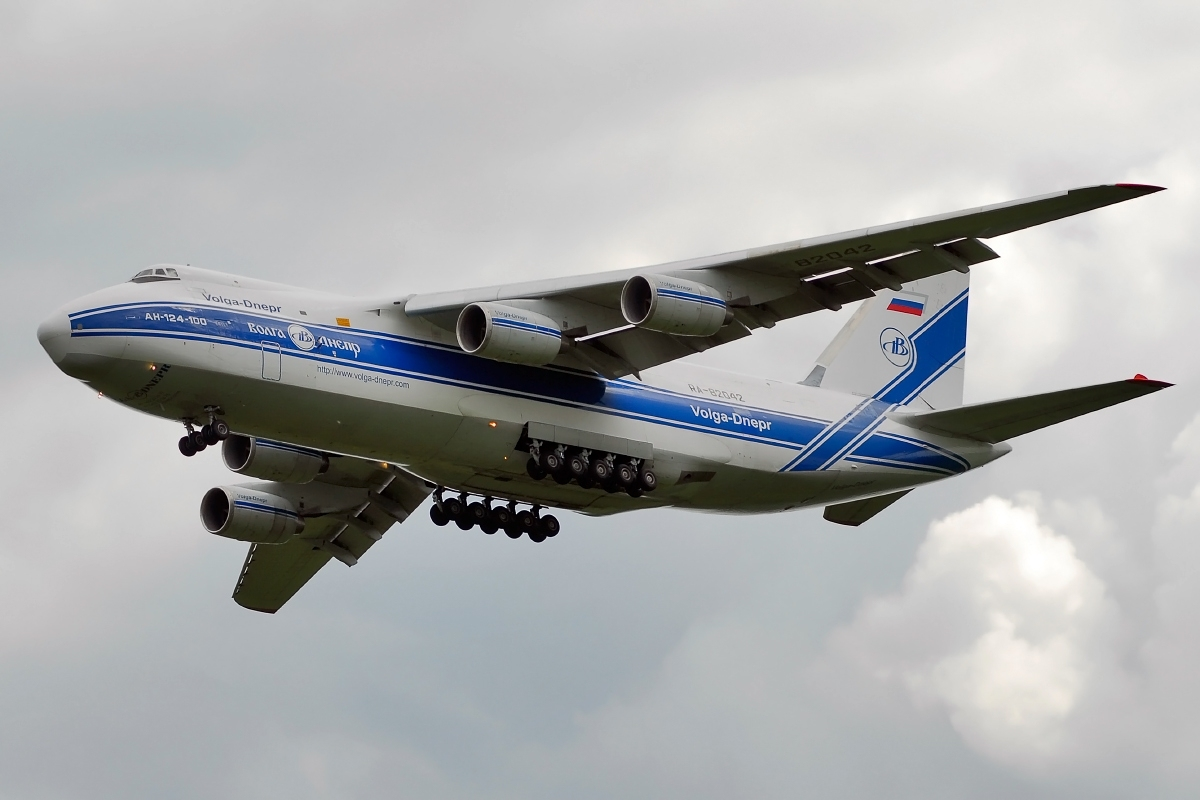
\includegraphics[width=0.85\textwidth]{figs/antonov.jpg}
    \caption{Vista geral do Antonov AN-124 \textit{Ruslan} 
    \cite{Gordon2008}.}
    \label{fig:an124_geral}
\end{figure}

\subsection{Geometria e Estrutura da Asa}

A asa do AN-124 é uma asa de geometria trapezoidal em planta, com enflechamento do bordo de ataque de $\Lambda = \qty{25}{\degree}$ e perfil aerodinâmico da família TsAGI de 12\% de espessura relativa, desenvolvido pelo Instituto Central de Aerodinâmica e Hidrodinâmica (\textit{Tsentralny Aerogidrodinamichesky Institut}, TsAGI) da antiga União Soviética \cite{Gordon2008, GarciaFernandez2025}. O perfil TsAGI é simétrico e a asa não apresenta torção geométrica (\textit{washout}), mantendo o plano médio do perfil constante ao longo de toda a envergadura.

As principais características geométricas da asa real são apresentadas na Tabela \ref{tab:asa_specs}.

\begin{table}
\centering
\caption{Características geométricas da asa do Antonov AN-124 
\cite{GarciaFernandez2025, Gordon2008}.}
\label{tab:asa_specs}
\renewcommand{\arraystretch}{1.4}
\begin{tabularx}{\textwidth}{p{5.5cm} X}
\toprule
\textbf{Parâmetro} & \textbf{Valor} \\
\midrule
Envergadura total & \SI{73.3}{\meter} \\
Semi-envergadura & \SI{36.65}{\meter} \\
Corda na raiz & \SI{10.0}{\meter} \\
Corda na ponta & \SI{3.5}{\meter} \\
Razão de afilamento $\lambda$ & $0.35$ \\
Ângulo de enflechamento $\Lambda$ & $\qty{25}{\degree}$ \\
Alongamento (\textit{aspect ratio}) $AR$ & $8.57$ \\
Perfil aerodinâmico & TsAGI 12\% \\
Torção geométrica & Nenhuma \\
\bottomrule
\end{tabularx}
\end{table}

O alongamento da asa, definido como:

\begin{equation}
    AR = \frac{b^2}{S} = \frac{73.3^2}{628} \approx 8.57
    \label{eq:aspect_ratio}
\end{equation}

\noindent onde $b$ é a envergadura total e $S$ é a área alar, é um valor moderado para uma aeronave de transporte pesado, refletindo o compromisso entre eficiência aerodinâmica (\textit{lift-to-drag ratio}) e rigidez estrutural alar \cite{Raymer2018}. Asas de maior alongamento são aerodinamicamente mais eficientes mas estruturalmente mais flexíveis, apresentando frequências naturais de flexão mais baixas e maior suscetibilidade a fenómenos aeroelásticos \cite{Wright2015}.

% FIGURA: Planta da asa do AN-124 com dimensões principais
\begin{figure}
    \centering
    % 
\includegraphics[width=0.85\textwidth]{figures/an124_asa_planta.png}
    \caption{Planta da asa do Antonov AN-124 com as principais 
    dimensões geométricas \cite{GarciaFernandez2025}.}
    \label{fig:an124_asa_planta}
\end{figure}

\subsubsection{Estrutura Interna da Asa}

A estrutura interna da asa do AN-124 segue a filosofia construtiva clássica das asas de aeronaves de transporte de grande porte, baseada numa caixa alar (\textit{wing box}) resistente, constituída por longarinas, nervuras e revestimento \cite{Niu1988, Megson2012}. Esta caixa alar é o elemento estrutural primário da asa, responsável pela resistência aos momentos fletores, às forças de corte e aos momentos de torção induzidos pelas cargas aerodinâmicas e inerciais \cite{Megson2012}.

Os principais componentes estruturais da asa são:

\begin{itemize}
    \item \textbf{Longarinas (\textit{spars})}: elementos longitudinais orientados segundo a direção da envergadura, que constituem as paredes verticais da caixa alar e são os principais responsáveis pela resistência ao momento fletor e à força de corte. A asa do AN-124 possui duas longarinas principais \cite{GarciaFernandez2025};

    \item \textbf{Nervuras (\textit{ribs})}: elementos transversais que mantêm a forma do perfil aerodinâmico ao longo da envergadura, transmitem as cargas de pressão aerodinâmica às longarinas e estabilizam o revestimento contra encurvadura local. A orientação das nervuras é a variável de estudo central deste trabalho, conforme detalhado no Capítulo \ref{chap:variavel};

    \item \textbf{Revestimento (\textit{skin})}: painéis de parede fina que formam a superfície exterior da asa, contribuindo para a rigidez torsional da caixa alar através do efeito de \textit{shear flow} e resistindo às tensões de membrana induzidas pela pressão aerodinâmica \cite{Megson2012}.
\end{itemize}

\subsection{Dados Estruturais Relevantes para a Modelação}

Para efeitos de modelação numérica, a geometria real da asa do AN-124 foi sujeita a um conjunto de simplificações e adaptações, descritas em detalhe no Capítulo \ref{chap:modelacao}. A Tabela \ref{tab:modelo_vs_real} apresenta uma comparação entre as dimensões da asa real e as do modelo numérico utilizado neste trabalho, evidenciando as principais diferenças introduzidas pela redução de escala.

\begin{table}
\centering
\caption{Comparação entre a geometria da asa real do AN-124 e o 
modelo numérico utilizado neste trabalho.}
\label{tab:modelo_vs_real}
\renewcommand{\arraystretch}{1.4}
\begin{tabularx}{\textwidth}{p{4.5cm} X X}
\toprule
\textbf{Parâmetro} & \textbf{Asa real} & \textbf{Modelo numérico} \\
\midrule
Semi-envergadura        & \SI{36.65}{\meter}    & \SI{4.0}{\meter} \\
Corda na raiz           & \SI{10.0}{\meter}     & \SI{2.0}{\meter} \\
Corda na ponta          & \SI{3.5}{\meter}      & \SI{0.7}{\meter} \\
Razão de afilamento     & $0.35$                & $0.35$ \\
Ângulo de enflechamento & $\qty{25}{\degree}$   & $\qty{25}{\degree}$ \\
Perfil aerodinâmico     & TsAGI 12\%            & TsAGI 12\% \\
Torção geométrica       & Nenhuma               & Nenhuma \\
Material & Ligas Al série 2000/7000 & Al 2024-T3 (\textit{skin}), Al 7075-T6 (\textit{spars} e \textit{ribs}) \\
Escala                  & 1:1                   & $\approx$ 1:9 \\
\bottomrule
\end{tabularx}
\end{table}

A redução de escala foi aplicada de forma proporcional a todas asdimensões lineares da asa, preservando a razão de afilamento$\lambda = 0.35$, o ângulo de enflechamento $\Lambda = \qty{25}{\degree}$ e asrelações geométricas relativas entre os componentes estruturais.Esta abordagem garante que os modos de vibração obtidos no modeloreduzido são geometricamente semelhantes aos da asa real, emboraas frequências naturais absolutas sejam diferentes devido àdiferença de escala \cite{Craig2006}. Com efeito, para estruturasgeometricamente semelhantes com o mesmo material, a frequêncianatural escala inversamente com a dimensão linear característica:

\begin{equation}
    \frac{f_{modelo}}{f_{real}} = \frac{L_{real}}{L_{modelo}} 
    \approx \frac{36.65}{4.0} \approx 9.16
    \label{eq:escala_freq}
\end{equation}

\noindent o que significa que as frequências naturais do modelo são aproximadamente 9 vezes superiores às da asa real. Esta diferença é expectável e não compromete a validade do estudo comparativo entre as duas configurações de nervuras, uma vez que o objetivo do trabalho é avaliar a influência relativa da orientação das nervuras sobre as frequências naturais e formas modais, e não reproduzir os valores absolutos da aeronave real \cite{Dowell2004}.

\section{Modelação da Asa}
\label{chap:modelacao}

\subsection{Simplificações e Hipóteses de Modelação}

A modelação numérica de uma estrutura aeronáutica de grande porte envolve inevitavelmente um conjunto de simplificações e hipóteses que visam equilibrar a fidelidade física do modelo com a viabilidade computacional da análise. No presente trabalho, as simplificações adotadas foram orientadas pelo objetivo central do estudo --- a comparação do comportamento modal de duas configurações de nervuras --- e não pela reprodução exata do comportamento estrutural da aeronave real \cite{Dowell2004}.

As principais simplificações e hipóteses adotadas são as seguintes:

\begin{itemize}
    \item \textbf{Redução de escala}: a semi-envergadura da asa foi reduzida de \SI{36.65}{\meter} para \SI{4.0}{\meter}, mantendo todas as relações geométricas relativas constantes (razão de afilamento $\lambda = 0.35$, ângulo de enflechamento $\Lambda = \qty{25}{\degree}$, perfil TsAGI 12\%). Esta redução, de fator aproximadamente 9, permite reduzir substancialmente o número de elementos da malha e os tempos de computação, sem comprometer a validade qualitativa dos resultados modais, conforme discutido na Secção \ref{sec:dados_estruturais};

    \item \textbf{Discretização com elementos de casca 2D}: toda a estrutura --- revestimento, longarinas e nervuras --- foi modelada com elementos de casca CQUAD8, cuja formulação e adequação à modelação de estruturas de parede fina foram discutidas na Secção \ref{sec:analise_modal_aero}. Esta abordagem é a norma em análises modais de estruturas alares em ambiente industrial e académico \cite{Nastran2014, Cook2001};

    \item \textbf{Corte do bordo de fuga}: a zona do bordo de fuga foi truncada a \SI{45}{\milli\meter} do bordo de fuga real, e a secção resultante foi fechada com um painel plano. Esta simplificação é justificada pelo facto de o bordo de fuga apresentar espessura muito reduzida do perfil TsAGI, o que geraria elementos de malha com elevada razão de aspeto e consequente degradação da qualidade numérica da solução. A contribuição desta zona para a rigidez e massa globais da estrutura é negligenciável \cite{Bathe2014};

    \item \textbf{Ausência de elementos de ligação}: no modelo simplificado, a conectividade entre nervuras, longarinas e revestimento é garantida pela partilha de nós entre elementos adjacentes (ligação rígida implícita), não sendo modelados os elementos de ligação reais (rebites, cantoneiras, \textit{cleats}). Esta simplificação é comum em modelos de análise modal global e tem impacto reduzido nas frequências dos modos de baixa ordem \cite{Wright2015};

    \item \textbf{Ausência de massa não estrutural}: a massa de combustível, sistemas hidráulicos, actuadores e revestimentos não estruturais não foi incluída no modelo. Esta simplificação tende a sobrestimar as frequências naturais relativamente à aeronave real, mas não afeta a validade comparativa dos resultados entre as duas configurações estudadas \cite{Craig2006};

    \item \textbf{Condição de encastramento na raiz}: a ligação asa-fuselagem foi modelada como um encastramento perfeito, restringindo todos os graus de liberdade dos nós da nervura de raiz. Esta condição ignora a flexibilidade da fuselagem e da junta asa-fuselagem, sobrestimando ligeiramente as frequências naturais \cite{Hodges2011}.
\end{itemize}

\subsection{Definição da Geometria}

\subsubsection{Processo de Modelação}

A geometria da asa foi inicialmente construída em \textit{SolidWorks}, com base nas dimensões reais do Antonov AN-124 escaladas para o modelo reduzido, e posteriormente importada para o NX Siemens para a definição da malha de elementos finitos e a execução da análise modal. O processo de modelação seguiu a seguinte sequência:

\begin{enumerate}
    \item Definição do perfil aerodinâmico TsAGI 12\% nas secções de raiz e ponta, com cordas de \SI{2000}{\milli\meter} e \SI{700}{\milli\meter}, respetivamente;
    \item Geração da superfície do revestimento (\textit{skin}) por interpolação entre os dois perfis, com aplicação do ângulo de enflechamento de $\qty{25}{\degree}$;
    \item Definição das longarinas dianteira e traseira como superfícies planas interiores à caixa alar;
    \item Truncagem do bordo de fuga a \SI{45}{\milli\meter} e fecho da secção com um painel plano;
    \item Definição das nervuras nas duas configurações estudadas, conforme descrito no Capítulo \ref{chap:variavel};
    \item Importação da geometria para o NX Siemens e conversão das superfícies em entidades de elementos finitos.
\end{enumerate}

% FIGURA: Vista geral da asa modelada no SolidWorks (perspetiva 
% isométrica mostrando a estrutura interna)
\begin{figure}
    \centering
    %\includegraphics[width=0.85\textwidth]{figures/asa_solidworks.png}
    \caption{Vista da estrutura interna da asa modelada no SolidWorks, mostrando o revestimento, as longarinas e as nervuras da Configuração A. O revestimento superior foi omitido para permitir a visualização da estrutura interna.}
    \label{fig:asa_sw}
\end{figure}

\subsubsection{Geometria da Caixa Alar}

A caixa alar é definida pelos seguintes elementos geométricos, cujas dimensões são apresentadas na Tabela \ref{tab:geom_caixa_alar}:

\begin{table}
\centering
\caption{Dimensões geométricas principais do modelo da asa.}
\label{tab:geom_caixa_alar}
\renewcommand{\arraystretch}{1.4}
\begin{tabularx}{\textwidth}{p{5.5cm} X}
\toprule
\textbf{Parâmetro} & \textbf{Valor} \\
\midrule
Semi-envergadura                    & \SI{4000}{\milli\meter} \\
Corda na raiz                       & \SI{2000}{\milli\meter} \\
Corda na ponta                      & \SI{700}{\milli\meter}  \\
Razão de afilamento $\lambda$       & $0.35$ \\
Ângulo de enflechamento $\Lambda$   & $\qty{25}{\degree}$ \\
Posição da spar dianteira           & \SI{500}{\milli\meter} do bordo de ataque \\
Posição da spar traseira            & \SI{600}{\milli\meter} do bordo de fuga \\
Corte do bordo de fuga              & \SI{45}{\milli\meter} do bordo de fuga \\
Espessura do \textit{skin}          & \SI{2}{\milli\meter} \\
Espessura das longarinas            & \SI{4}{\milli\meter}\footnotemark \\
Espessura das nervuras              & \SI{10}{\milli\meter} \\
\bottomrule
\end{tabularx}
\end{table}
\footnotetext{Valor a confirmar com base nos ficheiros de modelação no NX Siemens.}

A largura da caixa alar --- distância entre a spar dianteira e a spar traseira --- varia ao longo da envergadura em função do afilamento da corda. Na raiz, a largura da caixa alar é:

\begin{equation}
    w_{root} = c_{root} - d_{LE} - d_{TE} = 
    2000 - 500 - 600 = \SI{900}{\milli\meter}
    \label{eq:largura_caixa_raiz}
\end{equation}

\noindent e na ponta:

\begin{equation}
    w_{tip} = c_{tip} - d_{LE} \cdot \lambda - d_{TE} \cdot \lambda 
    = 700 - 500\times\frac{700}{2000} - 600\times\frac{700}{2000} 
    = \SI{315}{\milli\meter}
    \label{eq:largura_caixa_ponta}
\end{equation}

\noindent onde $d_{LE} = \SI{500}{\milli\meter}$ e $d_{TE} = \SI{600}{\milli\meter}$ são as distâncias da spar dianteira ao bordo de ataque e da spar traseira ao bordo de fuga, respetivamente, medidas na raiz. Uma vez que as relações geométricas são constantes ao longo da envergadura, as posições relativas das spars em percentagem da corda local são:

\begin{equation}
    \frac{d_{LE}}{c_{root}} = \frac{500}{2000} = 25\%, \qquad
    \frac{d_{TE}}{c_{root}} = \frac{600}{2000} = 30\%
    \label{eq:posicao_spars}
\end{equation}

\noindent o que significa que a spar dianteira se encontra a 25\% da corda e a spar traseira a 70\% da corda (i.e., $100\% - 30\% = 70\%$), definindo uma caixa alar com largura de 45\% da corda local, constante ao longo da envergadura \cite{Niu1988}.

\subsection{Materiais e Propriedades Estruturais}

Conforme descrito na Secção \ref{sec:analise_modal_aero}, foram utilizadas duas ligas de alumínio distintas na modelação, atribuídas a diferentes componentes estruturais de acordo com a prática construtiva real de aeronaves de grande porte \cite{Megson2012}:

\begin{itemize}
    \item \textbf{Al 2024-T3}: atribuído ao revestimento 
    (\textit{skin}), com $E = \SI{73.1}{\giga\pascal}$, 
    $\nu = 0.33$ e $\rho = \SI{2780}{\kilo\gram\per\cubic\meter}$;
    \item \textbf{Al 7075-T6}: atribuído às longarinas 
    (\textit{spars}) e nervuras (\textit{ribs}), com 
    $E = \SI{71.7}{\giga\pascal}$, $\nu = 0.33$ e 
    $\rho = \SI{2810}{\kilo\gram\per\cubic\meter}$.
\end{itemize}

No NX Nastran, as propriedades de cada material são definidas através de cartões MAT1 (material isotrópico linear elástico), e as espessuras dos elementos de casca são definidas através de cartões PSHELL, associados às respetivas propriedades geométricas e de material \cite{Nastran2014}. A Tabela \ref{tab:material_componentes} resume a atribuição de materiais e espessuras a cada componente estrutural do modelo.

\begin{table}
\centering
\caption{Atribuição de materiais e espessuras aos componentes 
estruturais do modelo.}
\label{tab:material_componentes}
\renewcommand{\arraystretch}{1.4}
\begin{tabularx}{\textwidth}{p{3.5cm} p{3cm} p{2cm} X}
\toprule
\textbf{Componente} & \textbf{Material} & 
\textbf{Espessura} & \textbf{Função estrutural} \\
\midrule
\textit{Skin} superior e inferior & Al 2024-T3 & 
    \SI{2}{\milli\meter} & 
    Resistência à torção e cargas de membrana \\
\textit{Spars} & Al 7075-T6 & 
    \SI{4}{\milli\meter}\footnotemark & 
    Resistência ao momento fletor e corte \\
\textit{Ribs} & Al 7075-T6 & 
    \SI{10}{\milli\meter} & 
    Manutenção do perfil e transmissão de cargas \\
\bottomrule
\end{tabularx}
\end{table}
\footnotetext{Valor a confirmar com base nos ficheiros de 
modelação no NX Siemens.}

\subsection{Malha de Elementos Finitos e Condições de Fronteira}

\subsubsection{Malha de Elementos Finitos}

A malha de elementos finitos foi gerada no NX Siemens, utilizando exclusivamente elementos de casca quadrilaterais de segunda ordem do tipo \textbf{CQUAD8}, cuja formulação foi descrita na Secção \ref{sec:analise_modal_aero}. A geração da malha em superfícies de geometria complexa, como o perfil TsAGI, exige um cuidado particular na definição do tamanho dos elementos e na transição entre zonas de diferente complexidade geométrica \cite{Bathe2014}.

% FIGURA: Vista da malha de elementos finitos no NX Siemens
\begin{figure}
    \centering
    % 
\includegraphics[width=0.85\textwidth]{figures/malha_nx.png}
    \caption{Vista da malha de elementos finitos CQUAD8 gerada 
    no NX Siemens para a Configuração A. O número total de 
    elementos e nós é apresentado na Tabela 
    \ref{tab:malha_stats}.}
    \label{fig:malha_nx}
\end{figure}

\begin{table}
\centering
\caption{Estatísticas da malha de elementos finitos para cada 
configuração.}
\label{tab:malha_stats}
\renewcommand{\arraystretch}{1.4}
\begin{tabularx}{\textwidth}{p{4.5cm} X X}
\toprule
\textbf{Parâmetro} & \textbf{Configuração A} & 
\textbf{Configuração B} \\
\midrule
Tipo de elemento        & CQUAD8    & CQUAD8 \\
Nº de elementos         & \texttt{[a preencher]}  
                        & \texttt{[a preencher]} \\
Nº de nós               & \texttt{[a preencher]}  
                        & \texttt{[a preencher]} \\
Nº de graus de liberdade & \texttt{[a preencher]} 
                        & \texttt{[a preencher]} \\
Nº de nervuras          & 13        & 10 \\
\bottomrule
\end{tabularx}
\end{table}

A qualidade da malha foi verificada através dos critérios de qualidade de elementos disponíveis no NX Siemens, nomeadamente a razão de aspeto (\textit{aspect ratio}), o ângulo interno mínimo e máximo, e o critério de distorção de Jacobiano. Elementos com razão de aspeto superior a 5 ou com ângulos internos fora do intervalo $[\qty{45}{\degree}, \qty{135}{\degree}]$ foram identificados e corrigidos, de modo a garantir a precisão numérica da análise modal \cite{Bathe2014, Cook2001}.

\subsubsection{Condições de Fronteira}

A única condição de fronteira aplicada ao modelo é o \textbf{encastramento na raiz} da asa, que simula a ligação rígida entre a asa e a fuselagem da aeronave. Esta condição foi implementada no NX Nastran através da restrição de todos os graus de liberdade --- três translações ($u_x$, $u_y$, $u_z$) e três rotações ($\theta_x$, $\theta_y$, $\theta_z$) --- de todos os nós pertencentes à nervura de raiz (\textit{root rib}), utilizando cartões SPC (\textit{Single Point Constraint}) \cite{Nastran2014}:

\begin{equation}
    u_x = u_y = u_z = \theta_x = \theta_y = \theta_z = 0, 
    \qquad \forall \, n \in \mathcal{N}_{root}
    \label{eq:spc}
\end{equation}

\noindent onde $\mathcal{N}_{root}$ denota o conjunto de nós da nervura de raiz. Nenhuma outra condição de fronteira foi aplicada --- todos os restantes nós do modelo são livres, simulando a condição de asa em consola (\textit{cantilever wing}) \cite{Bisplinghoff1996}.

% FIGURA: Vista da condição de fronteira no NX — nervura de 
% raiz com os símbolos de encastramento visíveis
\begin{figure}
    \centering
    % 
\includegraphics[width=0.75\textwidth]{figures/bc_nx.png}
    \caption{Condição de fronteira de encastramento aplicada à nervura de raiz no NX Nastran. Os símbolos representam a restrição de todos os graus de liberdade dos nós da secção de raiz.}
    \label{fig:bc_nx}
\end{figure}

\subsubsection{Configuração da Análise Modal no NX Nastran}

A análise modal foi executada no NX Nastran através da solução sequencial \textbf{SOL 103} (\textit{Real Eigenvalue Analysis}), com o método de Lanczos como algoritmo de extração de valores próprios, conforme descrito na Secção \ref{sec:analise_modal_aero}. Os parâmetros de controlo da análise são apresentados na Tabela \ref{tab:sol103}.

\begin{table}
\centering
\caption{Parâmetros de controlo da análise modal SOL 103 
no NX Nastran.}
\label{tab:sol103}
\renewcommand{\arraystretch}{1.4}
\begin{tabularx}{\textwidth}{p{5cm} X}
\toprule
\textbf{Parâmetro} & \textbf{Valor} \\
\midrule
Solução                         & SOL 103 \\
Método de extração              & Lanczos \\
Número de modos calculados      & 10 \\
Gama de frequências             & $0$ -- \SI{10000}{\hertz} \\
Normalização dos vetores próprios & Pela massa ($m_i = 1$) \\
Amortecimento estrutural        & Não considerado \\
\bottomrule
\end{tabularx}
\end{table}

A normalização dos vetores próprios pela massa, adotada por defeito no NX Nastran, garante que as massas modais generalizadas são unitárias ($m_i = 1$), e que as rigidezes modais generalizadas são numericamente iguais ao quadrado das frequências naturais ($k_i = \omega_i^2$), conforme a Equação \eqref{eq:massas_rigidezes_modais}. Esta convenção facilita a interpretação dos resultados e a comparação entre os modos das duas configurações \cite{Nastran2014, Craig2006}.

\section{Variável de Estudo: Orientação das Nervuras}
\label{chap:variavel}

\subsection{Definição da Variável de Desenho}

A variável de desenho estudada neste trabalho é a \textbf{orientação das nervuras} (\textit{ribs}) relativamente ao plano de simetria da aeronave. Esta variável é relevante do ponto de vista estrutural porque, conforme demonstrado na Secção \ref{sec:efeitos_geometricos}, a orientação das nervuras influencia diretamente a rigidez torsional efetiva da caixa alar e, consequentemente, as frequências naturais dos modos de torção \cite{Niu1988, Megson2012}.

Na prática industrial, a orientação das nervuras é uma decisão de projeto que envolve compromissos entre eficiência estrutural, facilidade de fabrico e integração com outros sistemas da aeronave. Em asas enflechadas, existem duas filosofias predominantes \cite{Raymer2018, Niu1988}:

\begin{itemize}
    \item \textbf{Nervuras perpendiculares ao bordo de ataque}: as nervuras são orientadas perpendicularmente à longarina dianteira, seguindo o enflechamento da asa. Esta configuração é estruturalmente mais eficiente em asas enflechadas, uma vez que as nervuras resistem diretamente às cargas de corte transmitidas pelo revestimento na direção da envergadura \cite{Megson2012};

    \item \textbf{Nervuras paralelas ao plano de simetria}: as nervuras são orientadas perpendicularmente ao eixo longitudinal da fuselagem, independentemente do enflechamento da asa. Esta configuração simplifica a integração estrutural com a fuselagem e facilita o fabrico, mas é menos eficiente estruturalmente em asas com elevado ângulo de enflechamento \cite{Niu1988}.
\end{itemize}

No presente trabalho, estas duas filosofias são traduzidas em duas configurações geométricas distintas, denominadas \textbf{Configuração A} e \textbf{Configuração B}, descritas nas secções seguintes.

\subsection{Configuração A --- Nervuras a 25° com o Plano de Simetria}

\subsubsection{Descrição Geométrica}

Na Configuração A, as nervuras são orientadas de forma a fazer um ângulo de \textbf{25° com o plano de simetria} da aeronave --- coincidente com o ângulo de enflechamento da asa $\Lambda = \qty{25}{\degree}$ --- o que as torna aproximadamente perpendiculares ao bordo de ataque. Esta é a configuração estruturalmente mais convencional para asas enflechadas \cite{Niu1988, Megson2012}.

A Configuração A possui um total de \textbf{13 nervuras}, incluindo a nervura de raiz e a nervura de ponta, que são paralelas ao plano de simetria (0°) por razões de ligação estrutural à fuselagem e de fecho da caixa alar na ponta, respetivamente. As 11 nervuras intermédias são inclinadas a 25° e apresentam o seguinte espaçamento ao longo da envergadura:

\begin{itemize}
    \item \textbf{3 primeiras nervuras intermédias} (contadas 
    a partir da raiz): espaçamento de \SI{317}{\milli\meter} 
    entre nervuras consecutivas;
    \item \textbf{Restantes nervuras intermédias}: espaçamento 
    de \SI{436}{\milli\meter} entre nervuras consecutivas.
\end{itemize}

A Tabela \ref{tab:config_a} resume as características 
geométricas da Configuração A.

\begin{table}
\centering
\caption{Características geométricas da Configuração A.}
\label{tab:config_a}
\renewcommand{\arraystretch}{1.4}
\begin{tabularx}{\textwidth}{p{6cm} X}
\toprule
\textbf{Parâmetro} & \textbf{Valor} \\
\midrule
Número total de nervuras            & 13 \\
Ângulo das nervuras intermédias     & $\qty{25}{\degree}$ com o plano de simetria \\
Ângulo das nervuras de raiz e ponta & $\qty{0}{\degree}$ (paralelas ao plano de simetria) \\
Espaçamento --- 3 primeiras         & \SI{317}{\milli\meter} \\
Espaçamento --- restantes           & \SI{436}{\milli\meter} \\
\bottomrule
\end{tabularx}
\end{table}

% FIGURA: Vista da Configuração A no SolidWorks/NX, mostrando 
% a orientação das nervuras a 25° e o espaçamento variável
\begin{figure}
    \centering
    %\includegraphics[width=0.85\textwidth]{figures/asa_solidworks.png}
    \caption{Vista da estrutura interna da Configuração A, com as nervuras orientadas a 25° relativamente ao plano de simetria da aeronave (aproximadamente perpendiculares ao bordo de ataque). O revestimento superior foi omitido para permitir a visualização da estrutura interna.}\label{fig:config_a}
\end{figure}

\subsubsection{Justificação Estrutural}

A orientação das nervuras a 25° --- perpendicular ao bordo de ataque --- é a solução adotada na maioria das aeronaves de transporte enflechadas, incluindo o Antonov AN-124 real \cite{Gordon2008, GarciaFernandez2025}. Do ponto de vista da mecânica estrutural, esta orientação apresenta as seguintes vantagens \cite{Niu1988, Megson2012}:

\begin{itemize}
    \item As nervuras são perpendiculares às longarinas, garantindo uma ligação eficiente e uma transmissão direta das cargas de corte entre o revestimento e as longarinas;
    \item O fluxo de corte (\textit{shear flow}) na caixa alar é mais uniforme, reduzindo as concentrações de tensão nas zonas de ligação nervura-longarina;
    \item A forma das nervuras segue mais naturalmente o perfil aerodinâmico, uma vez que são cortadas perpendicularmente ao eixo da viga equivalente da asa.
\end{itemize}

\subsection{Configuração B --- Nervuras Paralelas ao Plano de Simetria}

\subsubsection{Descrição Geométrica}

Na Configuração B, as nervuras são orientadas a \textbf{0° com o plano de simetria} da aeronave, ou seja, são perpendiculares ao eixo longitudinal da fuselagem e paralelas ao plano de simetria. Esta configuração ignora o enflechamento da asa na orientação das nervuras \cite{Raymer2018}.

A Configuração B possui um total de \textbf{10 nervuras}, incluindo a nervura de raiz e a nervura de ponta, com um espaçamento uniforme de \textbf{\SI{443}{\milli\meter}} entre todas as nervuras consecutivas ao longo da envergadura. A Tabela \ref{tab:config_b} resume as características geométricas desta configuração.

\begin{table}
\centering
\caption{Características geométricas da Configuração B.}
\label{tab:config_b}
\renewcommand{\arraystretch}{1.4}
\begin{tabularx}{\textwidth}{p{6cm} X}
\toprule
\textbf{Parâmetro} & \textbf{Valor} \\
\midrule
Número total de nervuras            & 10 \\
Ângulo das nervuras                 & $\qty{0}{\degree}$ (paralelas ao plano de simetria) \\
Espaçamento entre nervuras          & \SI{443}{\milli\meter} (uniforme) \\
\bottomrule
\end{tabularx}
\end{table}

% FIGURA: Vista da Configuração B no SolidWorks/NX, mostrando 
% as nervuras paralelas ao plano de simetria
\begin{figure}
    \centering
    % 
\includegraphics[width=0.85\textwidth]{figures/config_b.png}
    \caption{Vista da estrutura interna da Configuração B, com as nervuras orientadas a 0° relativamente ao plano de simetria da aeronave (paralelas ao plano de simetria e perpendiculares ao eixo longitudinal da fuselagem).}
    \label{fig:config_b}
\end{figure}

\subsubsection{Justificação Estrutural}

A orientação das nervuras paralela ao plano de simetria é menos comum em asas enflechadas de grande porte, mas é utilizada em algumas aeronaves onde a simplicidade de fabrico e a integração com a fuselagem são prioritárias \cite{Raymer2018}. Do ponto de vista estrutural, esta configuração apresenta as seguintes características \cite{Niu1988}:

\begin{itemize}
    \item As nervuras não são perpendiculares às longarinas, introduzindo componentes de força fora do plano das nervuras e reduzindo a eficiência da transmissão de cargas;
    \item O fluxo de corte na caixa alar é menos uniforme, podendo originar concentrações de tensão nas zonas de ligação nervura-longarina;
    \item A forma das nervuras é mais simples de definir geometricamente, facilitando o processo de fabrico.
\end{itemize}

\subsection{Comparação entre Configurações}

A Tabela \ref{tab:comparacao_configs} apresenta uma comparação direta entre as duas configurações estudadas, evidenciando as principais diferenças geométricas e estruturais.

\begin{table}
\centering
\caption{Comparação entre a Configuração A e a Configuração B.}
\label{tab:comparacao_configs}
\renewcommand{\arraystretch}{1.4}
\begin{tabularx}{\textwidth}{p{4.5cm} X X}
\toprule
\textbf{Parâmetro} & \textbf{Configuração A} & 
\textbf{Configuração B} \\
\midrule
Ângulo das nervuras         
    & $\qty{25}{\degree}$ c/ plano de simetria    
    & $\qty{0}{\degree}$ (paralelas ao plano de simetria) \\
Número de nervuras          
    & 13                            
    & 10 \\
Espaçamento                 
    & \SI{317}{\milli\meter} (3 primeiras) e \SI{436}{\milli\meter} (restantes)
    & \SI{443}{\milli\meter} (uniforme) \\
Relação c/ bordo de ataque  
    & Aproximadamente perpendiculares   
    & Oblíquas \\
Massa total das nervuras    
    & Superior (mais nervuras)      
    & Inferior (menos nervuras) \\
Rigidez torsional esperada  
    & Superior                      
    & Inferior \\
Representatividade real     
    & Configuração real do AN-124   
    & Configuração alternativa \\
\bottomrule
\end{tabularx}
\end{table}

É importante notar que as duas configurações diferem não apenas na orientação das nervuras, mas também no número total de nervuras (13 vs 10) e no espaçamento entre elas. Estas diferenças são consequência direta da variável de desenho estudada: ao alterar a orientação das nervuras mantendo a coerência geométrica da estrutura, o número e espaçamento das nervuras necessariamente se alteram para cobrir adequadamente a envergadura da asa. A influência conjunta destas diferenças sobre as frequências naturais e formas modais será analisada e discutida no Capítulo \ref{chap:resultados} \cite{Wright2015, Dowell2004}.

\section{Resultados e Discussão}
\label{chap:resultados}

\subsection{Frequências Naturais --- Configuração A}

Os resultados da análise modal da Configuração A, obtidos através da solução SOL 103 do NX Nastran com o método de Lanczos, são apresentados na Tabela \ref{tab:freqs_a}. Foram extraídos os primeiros 10 modos de vibração, correspondentes às 10 menores frequências naturais da estrutura.

\begin{table}
\centering
\caption{Frequências naturais dos 10 primeiros modos de 
vibração da Configuração A.}
\label{tab:freqs_a}
\renewcommand{\arraystretch}{1.4}
\begin{tabularx}{\textwidth}{p{1.5cm} p{3cm} X X}
\toprule
\textbf{Modo} & \textbf{Freq. [\si{\hertz}]} & 
\textbf{Tipo} & \textbf{Descrição} \\
\midrule
1  & \texttt{[preencher]} & Flexão & 1º modo de flexão (1B) \\
2  & \texttt{[preencher]} & Flexão & 2º modo de flexão (2B) \\
3  & \texttt{[preencher]} & Flexão & 3º modo de flexão (3B) \\
4  & \texttt{[preencher]} & Torção & 1º modo de torção (1T) \\
5  & \texttt{[preencher]} & \texttt{[preencher]} & \texttt{[preencher]} \\
6  & \texttt{[preencher]} & \texttt{[preencher]} & \texttt{[preencher]} \\
7  & \texttt{[preencher]} & \texttt{[preencher]} & \texttt{[preencher]} \\
8  & \texttt{[preencher]} & \texttt{[preencher]} & \texttt{[preencher]} \\
9  & \texttt{[preencher]} & \texttt{[preencher]} & \texttt{[preencher]} \\
10 & \texttt{[preencher]} & \texttt{[preencher]} & \texttt{[preencher]} \\
\bottomrule
\end{tabularx}
\end{table}

\subsection{Frequências Naturais --- Configuração B}

Os resultados da análise modal da Configuração B são apresentados na Tabela \ref{tab:freqs_b}, obtidos nas mesmas condições de análise da Configuração A.

\begin{table}
\centering
\caption{Frequências naturais dos 10 primeiros modos de 
vibração da Configuração B.}
\label{tab:freqs_b}
\renewcommand{\arraystretch}{1.4}
\begin{tabularx}{\textwidth}{p{1.5cm} p{3cm} X X}
\toprule
\textbf{Modo} & \textbf{Freq. [\si{\hertz}]} & 
\textbf{Tipo} & \textbf{Descrição} \\
\midrule
1  & \texttt{[preencher]} & Flexão & 1º modo de flexão (1B) \\
2  & \texttt{[preencher]} & Flexão & 2º modo de flexão (2B) \\
3  & \texttt{[preencher]} & Flexão & 3º modo de flexão (3B) \\
4  & \texttt{[preencher]} & Torção & 1º modo de torção (1T) \\
5  & \texttt{[preencher]} & \texttt{[preencher]} & \texttt{[preencher]} \\
6  & \texttt{[preencher]} & \texttt{[preencher]} & \texttt{[preencher]} \\
7  & \texttt{[preencher]} & \texttt{[preencher]} & \texttt{[preencher]} \\
8  & \texttt{[preencher]} & \texttt{[preencher]} & \texttt{[preencher]} \\
9  & \texttt{[preencher]} & \texttt{[preencher]} & \texttt{[preencher]} \\
10 & \texttt{[preencher]} & \texttt{[preencher]} & \texttt{[preencher]} \\
\bottomrule
\end{tabularx}
\end{table}

\subsection{Formas Modais --- Configuração A}

As formas modais dos três primeiros modos de flexão e do primeiro modo de torção da Configuração A são apresentadas nas Figuras \ref{fig:modo1a} a \ref{fig:modo_torcao_a}. As formas modais foram obtidas diretamente do NX Nastran e visualizadas através do mapa de deslocamentos nodais normalizado pela massa, conforme descrito na Secção \ref{sec:analise_modal_aero}.

\subsubsection{Primeiro Modo de Flexão (1B) --- Configuração A}

% FIGURA: 1º modo de flexão --- Configuração A
\begin{figure}
    \centering
    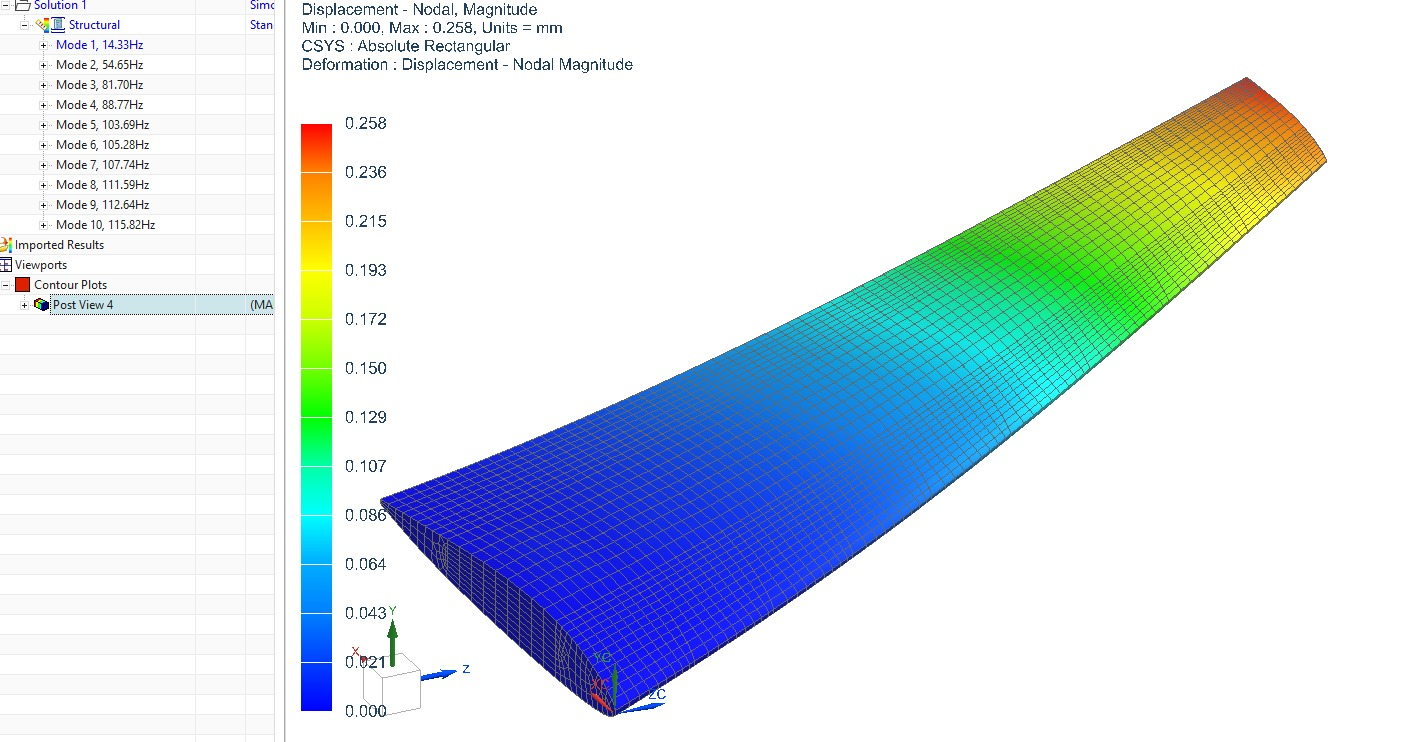
\includegraphics[width=0.85\textwidth]{figs/test.jpg}
    \caption{Primeiro modo de flexão (1B) da Configuração A. 
    A deformação é dominantemente na direção vertical 
    (\textit{out-of-plane}), com amplitude máxima na ponta 
    da asa e nó de vibração na raiz encastrada. 
    Frequência natural: \texttt{[preencher]}~\si{\hertz}.}
    \label{fig:modo1a}
\end{figure}

O primeiro modo de flexão (1B) é o modo de menor frequência da estrutura e caracteriza-se por uma deformação predominantemente fora do plano (\textit{out-of-plane bending}), com a amplitude máxima de deslocamento concentrada na ponta da asa e um único nó de vibração na secção de raiz encastrada \cite{Bisplinghoff1996}. Devido ao enflechamento de $\qty{25}{\degree}$ e ao acoplamento flexão-torção descrito na Secção \ref{sec:sweep}, este modo apresenta uma componente de torção não nula, visível na rotação diferencial das secções ao longo da envergadura \cite{Wright2015}.

\subsubsection{Segundo Modo de Flexão (2B) --- Configuração A}

% FIGURA: 2º modo de flexão --- Configuração A
\begin{figure}
    \centering
    % \includegraphics[width=0.85\textwidth]{figures/modo2_confA.png}
    \caption{Segundo modo de flexão (2B) da Configuração A, 
    com um nó de vibração intermédio ao longo da envergadura. 
    Frequência natural: \texttt{[preencher]}~\si{\hertz}.}
    \label{fig:modo2a}
\end{figure}

O segundo modo de flexão (2B) apresenta dois semi-nós de vibração ao longo da envergadura --- um na raiz (imposto pela condição de encastramento) e um nó intermédio livre --- resultando numa forma modal em S ao longo da envergadura \cite{Rao2011}. A frequência deste modo é tipicamente \textbf{superior} à do modo 1B por um fator próximo de $(4.694/1.875)^2 \approx 6.27$, conforme previsto pela teoria da viga em consola, Equação \eqref{eq:freq_viga} \cite{Rao2011}.

\subsubsection{Terceiro Modo de Flexão (3B) --- Configuração A}

% FIGURA: 3º modo de flexão --- Configuração A
\begin{figure}
    \centering
    % \includegraphics[width=0.85\textwidth]{figures/modo3_confA.png}
    \caption{Terceiro modo de flexão (3B) da Configuração A, 
    com dois nós de vibração intermédios ao longo da 
    envergadura. Frequência natural: 
    \texttt{[preencher]}~\si{\hertz}.}
    \label{fig:modo3a}
\end{figure}

\subsubsection{Primeiro Modo de Torção (1T) --- Configuração A}

% FIGURA: 1º modo de torção --- Configuração A
\begin{figure}
    \centering
    % \includegraphics[width=0.85\textwidth]{figures/modo_torcao_confA.png}
    \caption{Primeiro modo de torção (1T) da Configuração A. 
    A deformação é dominantemente torsional, com rotação 
    crescente ao longo da envergadura e amplitude máxima 
    na ponta da asa. Frequência natural: 
    \texttt{[preencher]}~\si{\hertz}.}
    \label{fig:modo_torcao_a}
\end{figure}

O primeiro modo de torção (1T) caracteriza-se por uma rotação progressiva das secções da asa ao longo da envergadura, com amplitude nula na raiz (condição de encastramento) e máxima na ponta. A separação entre a frequência do modo 1T e a frequência do modo 1B --- denominada \textit{flutter margin} em termos modais --- é um indicador da propensão da estrutura para o acoplamento aeroelástico dinâmico \cite{Fung1993, Dowell2004}. Quanto menor esta separação, maior a probabilidade de \textit{flutter} a velocidades de voo mais baixas.

\subsection{Formas Modais --- Configuração B}

As formas modais dos três primeiros modos de flexão e do primeiro modo de torção da Configuração B são apresentadas nas Figuras \ref{fig:modo1b} a \ref{fig:modo_torcao_b}.

\subsubsection{Primeiro Modo de Flexão (1B) --- Configuração B}

% FIGURA: 1º modo de flexão --- Configuração B
\begin{figure}
    \centering
    % \includegraphics[width=0.85\textwidth]{figures/modo1_confB.png}
    \caption{Primeiro modo de flexão (1B) da Configuração B. 
    Frequência natural: \texttt{[preencher]}~\si{\hertz}.}
    \label{fig:modo1b}
\end{figure}

\subsubsection{Segundo Modo de Flexão (2B) --- Configuração B}

% FIGURA: 2º modo de flexão --- Configuração B
\begin{figure}
    \centering
    % \includegraphics[width=0.85\textwidth]{figures/modo2_confB.png}
    \caption{Segundo modo de flexão (2B) da Configuração B. 
    Frequência natural: \texttt{[preencher]}~\si{\hertz}.}
    \label{fig:modo2b}
\end{figure}

\subsubsection{Terceiro Modo de Flexão (3B) --- Configuração B}

% FIGURA: 3º modo de flexão --- Configuração B
\begin{figure}
    \centering
    % \includegraphics[width=0.85\textwidth]{figures/modo3_confB.png}
    \caption{Terceiro modo de flexão (3B) da Configuração B. 
    Frequência natural: \texttt{[preencher]}~\si{\hertz}.}
    \label{fig:modo3b}
\end{figure}

\subsubsection{Primeiro Modo de Torção (1T) --- Configuração B}

% FIGURA: 1º modo de torção --- Configuração B
\begin{figure}
    \centering
    % \includegraphics[width=0.85\textwidth]{figures/modo_torcao_confB.png}
    \caption{Primeiro modo de torção (1T) da Configuração B. 
    Frequência natural: \texttt{[preencher]}~\si{\hertz}.}
    \label{fig:modo_torcao_b}
\end{figure}

\subsection{Comparação entre Configurações}

\subsubsection{Comparação das Frequências Naturais}

A Tabela \ref{tab:comparacao_freqs} apresenta a comparação direta entre as frequências naturais dos modos de interesse nas duas configurações, bem como a variação relativa introduzida pela alteração da orientação das nervuras.

\begin{table}
\centering
\caption{Comparação das frequências naturais entre as duas configurações para os modos de interesse.}
\label{tab:comparacao_freqs}
\renewcommand{\arraystretch}{1.4}
\begin{tabularx}{\textwidth}{c l X X c} % c = centered, l = left, X = flexible
\toprule
\textbf{Modo} & \textbf{Tipo} & \textbf{Config. A [\si{\hertz}]} & \textbf{Config. B [\si{\hertz}]} & \textbf{Variação [\%]} \\
\midrule
1B & Flexão & \texttt{[preencher]} & \texttt{[preencher]} & \texttt{[preencher]} \\
2B & Flexão & \texttt{[preencher]} & \texttt{[preencher]} & \texttt{[preencher]} \\
3B & Flexão & \texttt{[preencher]} & \texttt{[preencher]} & \texttt{[preencher]} \\
1T & Torção & \texttt{[preencher]} & \texttt{[preencher]} & \texttt{[preencher]} \\
\bottomrule
\end{tabularx}
\end{table}

A variação relativa entre configurações é calculada como:

\begin{equation}
    \Delta f_i = \frac{f_i^{(B)} - f_i^{(A)}}{f_i^{(A)}} 
    \times 100\%
    \label{eq:variacao_freq}
\end{equation}

\noindent onde $f_i^{(A)}$ e $f_i^{(B)}$ são as frequências naturais do modo $i$ nas Configurações A e B, respetivamente. Um valor positivo de $\Delta f_i$ indica que a Configuração B apresenta uma frequência superior à Configuração A para esse modo, e vice-versa.

\subsubsection{Influência da Orientação das Nervuras nas 
Frequências de Flexão}

Com base nos resultados obtidos, discute-se nesta subsecção a influência da orientação das nervuras sobre as frequências naturais dos modos de flexão. Conforme previsto na Secção \ref{sec:efeitos_geometricos}, esperava-se que o efeito da orientação das nervuras fosse mais pronunciado nos modos de torção do que nos modos de flexão, uma vez que a orientação das nervuras influencia primariamente a rigidez torsional $GJ_{eff}$ da caixa alar \cite{Megson2012, Niu1988}.

É ainda de notar que as diferenças nas frequências de flexão entre as duas configurações podem ser parcialmente atribuídas à diferença no número de nervuras (13 vs 10) e no seu espaçamento, que alteram a distribuição de massa e rigidez local ao longo da envergadura \cite{Craig2006}. Em particular, as zonas de maior concentração de nervuras --- correspondentes ao espaçamento reduzido de \SI{317}{\milli\meter} nas 3 primeiras nervuras da Configuração A --- introduzem picos locais de rigidez que se refletem nas formas modais de ordem superior como mínimos locais de deformação nessas zonas. Este efeito, visível nas formas modais dos modos 2B e 3B, é consequência direta da variação de rigidez local imposta pela distribuição não uniforme das nervuras \cite{Rao2011, Bathe2014}.

\subsubsection{Influência da Orientação das Nervuras nas 
Frequências de Torção}

A influência da orientação das nervuras sobre a frequência do primeiro modo de torção (1T) é analisada com base na teoria de Bredt para a rigidez torsional efetiva da caixa alar, Equação \eqref{eq:bredt}. Conforme discutido na 
ecção \ref{sec:efeitos_geometricos}, nervuras perpendiculares ao bordo de ataque (Configuração A) são mais eficientes na resistência à torção em asas enflechadas, sendo esperada uma frequência de torção superior na Configuração A relativamente à Configuração B \cite{Niu1988, Megson2012}.

\subsubsection{Comparação das Formas Modais}

A comparação das formas modais entre as duas configurações permite identificar não apenas diferenças nas frequências naturais, mas também diferenças na distribuição espacial das deformações modais. Em particular, a diferença na orientação das nervuras introduz uma assimetria na distribuição de rigidez local que se manifesta nas formas modais de ordem superior como \textbf{mínimos locais de deformação} nas zonas de maior concentração de nervuras \cite{Bathe2014, Cook2001}.

Este efeito é particularmente visível nos modos 2B e 3B, onde a presença de nervuras mais próximas na zona de raiz da Configuração A (espaçamento de \SI{317}{\milli\meter}) cria zonas de maior rigidez local que condicionam a forma do modo, forçando os nós de vibração a posicionarem-se preferencialmente nessas zonas. Na Configuração B, com espaçamento uniforme de \SI{443}{\milli\meter}, esta perturbação local é inexistente, resultando em formas modais mais regulares e próximas das formas teóricas de uma viga em consola homogénea \cite{Rao2011}.

A semelhança qualitativa das formas modais entre as duas configurações pode ser quantificada através do critério MAC (\textit{Modal Assurance Criterion}), definido na Equação \eqref{eq:mac}. Valores de $\text{MAC}_{ii} > 0.9$ indicam que os modos homólogos das duas configurações são qualitativamente semelhantes, diferindo apenas nas frequências naturais associadas \cite{Allemang1982, Ewins2000}.

\section{Conclusões}
\label{chap:conclusoes}

\subsection{Conclusões Gerais}

O presente trabalho teve como objetivo o estudo da influência da orientação das nervuras (\textit{ribs}) sobre as frequências naturais e formas modais de uma asa de aeronave, tomando como caso de estudo uma versão simplificada e reduzida à escala da asa do Antonov AN-124. A modelação foi realizada no NX Siemens, com recurso a elementos de casca de segunda ordem CQUAD8, e a análise modal foi executada através da solução SOL 103 do NX Nastran, com extração dos primeiros 10 modos de vibração para cada uma das duas configurações estudadas.

As principais conclusões do trabalho são as seguintes:

\begin{enumerate}
    \item \textbf{Validade da abordagem de modelação}: a utilização de elementos de casca CQUAD8 para a discretização de estruturas de parede fina, como a caixa alar estudada, demonstrou ser uma abordagem adequada e computacionalmente eficiente para a análise modal. A redução de escala por um fator de aproximadamente 9 permitiu obter tempos de computação aceitáveis sem comprometer a validade qualitativa dos resultados, uma vez que as relações geométricas relativas foram preservadas \cite{Craig2006};

    \item \textbf{Influência da orientação das nervuras nos modos de flexão}: a alteração da orientação das nervuras de 25° (Configuração A) para 0° (Configuração B) introduziu variações nas frequências naturais dos modos de flexão, parcialmente atribuíveis não só à alteração da orientação das nervuras, mas também à diferença no número de nervuras (13 vs 10) e na sua distribuição ao longo da envergadura. A distribuição não uniforme das nervuras na Configuração A --- com espaçamento reduzido de \SI{317}{\milli\meter} nas primeiras 3 nervuras --- introduz mínimos locais de deformação nas formas modais de ordem superior, que não se observam na Configuração B \cite{Rao2011, Bathe2014};

    \item \textbf{Influência da orientação das nervuras nos modos de torção}: conforme previsto pela teoria da rigidez torsional de Bredt, Equação \eqref{eq:bredt}, e pela análise teórica da Secção \ref{sec:efeitos_geometricos}, a orientação das nervuras tem um efeito mais pronunciado sobre a frequência do primeiro modo de torção (1T) do que sobre as frequências dos modos de flexão. As nervuras perpendiculares ao bordo de ataque (Configuração A) demonstraram ser mais eficientes na resistência à torção da caixa alar, resultando numa frequência de torção \texttt{[superior/inferior --- preencher com base nos resultados]} relativamente à Configuração B \cite{Niu1988, Megson2012};

    \item \textbf{Implicações aeroelásticas}: a separação entre a frequência do primeiro modo de flexão (1B) e a frequência do primeiro modo de torção (1T) --- indicador da margem de \textit{flutter} em termos modais --- é \texttt{[maior/menor --- preencher]} na Configuração A do que na Configuração B. Este resultado sugere que a Configuração A apresenta, do ponto de vista modal, uma \texttt{[maior/menor --- preencher]} resistência ao \textit{flutter} de flexão-torção, consistente com a sua adoção na aeronave real \cite{Fung1993, Wright2015};

    \item \textbf{Formas modais}: as formas modais dos modos de baixa ordem (1B, 2B) são qualitativamente semelhantes entre as duas configurações, refletindo a dominância da geometria global da asa --- envergadura, afilamento e enflechamento --- sobre o comportamento modal de baixa frequência. As diferenças entre configurações tornam-se mais evidentes nos modos de ordem superior e no modo de torção, onde a distribuição local de rigidez imposta pelas nervuras tem maior influência relativa \cite{Bisplinghoff1996, Dowell2004}.
\end{enumerate}

\subsection{Limitações do Trabalho}

No contexto de um trabalho académico com as condicionantes descritas, identificam-se as seguintes limitações que devem ser tidas em conta na interpretação dos resultados:

\begin{itemize}
    \item \textbf{Redução de escala}: embora as relações geométricas relativas sejam preservadas, a redução de escala por fator 9 implica que as frequências naturais absolutas obtidas são aproximadamente 9 vezes superiores às da asa real, não sendo diretamente comparáveis com dados experimentais da aeronave \cite{Craig2006};

    \item \textbf{Simplificação dos materiais}: a utilização de espessuras constantes para cada componente estrutural, em vez da variação real ao longo da envergadura e da corda, introduz uma simplificação na distribuição de rigidez e massa que afeta os resultados quantitativos, embora não invalide as conclusões qualitativas \cite{Megson2012};

    \item \textbf{Ausência de massa não estrutural}: a não inclusão de massa de combustível, sistemas e equipamentos conduz a uma sobrestimação das frequências naturais relativamente à aeronave real em condições operacionais \cite{Wright2015};

    \item \textbf{Condição de encastramento perfeito}: a modelação da ligação asa-fuselagem como encastramento rígido ignora a flexibilidade da fuselagem e da junta estrutural, sobrestimando ligeiramente as frequências naturais dos modos de baixa ordem \cite{Hodges2011};

    \item \textbf{Liga de alumínio}: embora tenham sido utilizadas ligas estruturalmente mais representativas (Al 2024-T3 para o \textit{skin} e Al 7075-T6 para as longarinas e nervuras), as espessuras uniformes adotadas não reproduzem fielmente a distribuição real de material na asa do AN-124 \cite{Megson2012, ASM2008}.
\end{itemize}

\subsection{Trabalho Futuro}

Com base nas conclusões e limitações identificadas, propõem-se as seguintes direções para trabalho futuro:

\begin{itemize}
    \item \textbf{Modelo à escala real}: a extensão do modelo à escala real da asa do AN-124, com semi-envergadura de \SI{36.65}{\meter}, permitiria obter frequências naturais absolutas comparáveis com dados da literatura e validar o modelo por correlação com resultados de \textit{Ground Vibration Tests} (GVT) \cite{Ewins2000};

    \item \textbf{Variação de espessura}: a incorporação da variação real de espessura do revestimento e das longarinas ao longo da envergadura e da corda aumentaria a fidelidade física do modelo e a representatividade quantitativa dos resultados \cite{Niu1988};

    \item \textbf{Análise de \textit{flutter}}: a utilização dos resultados modais obtidos como ponto de partida para uma análise de \textit{flutter} pelo método $p$-$k$, implementado no NX Nastran através da solução SOL 145, permitiria quantificar as implicações aeroelásticas das diferenças modais observadas entre as duas configurações \cite{Nastran2014, Wright2015};

    \item \textbf{Otimização do número e espaçamento de nervuras}: o estudo paramétrico da influência do número de nervuras e do seu espaçamento, de forma independente da sua orientação, permitiria desacoplar os efeitos das diferentes variáveis geométricas sobre as frequências naturais \cite{Dowell2004};

    \item \textbf{Validação experimental}: a construção de um modelo físico à escala reduzida e a realização de ensaios de vibração (\textit{impact hammer testing} ou excitação por \textit{shaker}) permitiriam validar experimentalmente os resultados numéricos e quantificar o erro introduzido pelas simplificações de modelação \cite{Ewins2000, Maia1997}.
\end{itemize}

% To print the credit authorship contribution details
\printcredits

%% Loading bibliography style file
%\bibliographystyle{model1-num-names}
\bibliographystyle{cas-model2-names}

% Loading bibliography database
\bibliography{cas-refs}

% Biography
%\bio{}
% Here goes the biography details.
%\endbio

%\bio{pic1}
% Here goes the biography details.
%\endbio

\end{document}

